% DIPLOMOVÁ PRÁCE
% ===============

\documentclass[11pt,twoside,a4paper]{book}
\usepackage[a4paper,width=15cm,height=23cm,twoside]{geometry}
\usepackage{amssymb}
\usepackage[utf8]{inputenc}
\usepackage[usenames,dvipsnames]{color}
\usepackage{graphicx}
\usepackage{subfig}
\captionsetup{labelfont={bf},margin=8pt,captionskip=13pt}
\usepackage[czech,english]{babel}
\usepackage[calcwidth]{titlesec}
\titleformat{\chapter}[display]{\normalfont\bf}{\titlerule[1pt]\vspace{1pt}\titlerule\vspace{1pc}\Huge\MakeUppercase{\chaptertitlename} \thechapter}{1pc}{\titlerule\vspace{1pc}\Huge}
\titleformat{\section}[hang]{\normalfont\bf}{\color{Gray}\LARGE\thesection}{0pt}{\linebreak\LARGE\raggedright}[{\vspace{1ex}\titlerule}]
\titleformat{\subsection}[hang]{\normalfont\bf}{\color{Gray}\large\thesubsection}{0pt}{\linebreak\Large\raggedright}[{\vspace{1ex}\titlerule}]
\titleformat{\subsubsection}[hang]{\normalfont\sc\bf}{\color{Gray}\large\thesubsubsection}{0pt}{\linebreak\large\raggedright}[{\vspace{1ex}\titlerule\sc}]
\usepackage{algorithmic}
\algsetup{indent=1em}
\usepackage{listings}
\lstset{
  columns=fullflexible,
  language=Java,
  numbers=left,
  frame=leftline, 
  rulesepcolor=\color{Gray},
  basicstyle=\small,
  numberstyle=\sc\footnotesize\color{Gray},
  commentstyle=\it\footnotesize\color{Gray}
}
\usepackage[
  pdftitle={Master's Thesis},
  pdfauthor={Bc.~Vojtěch~Hordějčuk},
  bookmarks=true,
  colorlinks=true,
  urlcolor=black,
  citecolor=black,
  linkcolor=black,
  unicode=true
]{hyperref}
\pagestyle{empty}
\setlength{\columnsep}{5pt}
\linespread{1.1}
\setcounter{tocdepth}{2}
\setcounter{secnumdepth}{3}
\parindent=1em
\parskip=1em plus 1em minus 0.7em
\def\MakeUppercase#1{{\it #1}}
\graphicspath{{figures//}}

\begin{document}

% Titulní stránka
% ===============

\cleardoublepage

\begin{center}

{\large Czech Technical University in Prague \\
Faculty of Electrical Engineering \\
Department of Computer Science and Engineering}

\vfill

\includegraphics[width=0.6\paperwidth]{ctu.pdf}

\vfill

{\large MASTER THESIS}

\vfill
\hrule
\vfill

{\LARGE
\bf Optimisation of Rectangular Shapes Placement \\
by Means of Evolutionary Algorithms}

{\LARGE Bc.~Vojtěch~Hordějčuk}

\vfill

{\em Supervisor}: {\small Ing.~Jiří~Kubalík,~Ph.D.}

{\em Study~Programme}: {\small Elektrotechnika~a~informatika,~strukturovaný,~magisterský}

{\em Field~of~Study}: {\small Výpočetní~technika, Softwarové~inženýrství}

\vfill

\today

\end{center}

% Poděkování a prohlášení
% =======================

\cleardoublepage
\vspace*{\fill}

\section*{Acknowledgements}

My supervisor, Mr.~Ing.~Jiří~Kubalík~Ph.D., for valuable advice and research insight.

\section*{Statement}

I hereby declare that I have completed this thesis independently and that I have listed all the literature and publications used within the research and work. I have no objections to usage of this work in compliance with Act~No~121/2000 Sb. (the Copyright~Act), as amended, and in compliance with copyright-related rights currently in force.

\bigskip
\bigskip

\noindent
Prague, \today \hfill \hbox to 70mm{\tiny\dotfill}

% Abstrakt
% ========

\cleardoublepage
\vspace*{\fill}

\section*{Abstract}

The aim of this work is to design and test an evolutionary algorithm that is capable of placing rectangular shapes onto the plane that the rectangle containing all modules is as small as possible. Under this modelling, real problems are considered, such as VLSI chip floorplanning, simple task planning or civil engineering. An evolutionary algorithm is used to optimise the floorplan represented as a tree (B*-Tree).

\section*{Abstrakt}

Cílem práce bylo navrhnout a otestovat evoluční algoritmus, který bude schopný rozmístit obdélníkové útvary na plochu tak, aby celková plocha obdélníku, který tyto útvary ohraničuje, byla co nejmenší. Úlohou je možné modelovat různé problémy reálného světa - například rozmisťování funkčních bloků na VLSI čip (tzv. floorplanning), jednoduché plánování či urbanistiku. K optimalizaci je použit iterativní evoluční algoritmus, pracující se stromovou reprezentací (B*-Tree).

% Obsah
% =====

\tableofcontents

% Kapitoly
% ========

\cleardoublepage
\setcounter{page}{1}
\pagestyle{headings}
\pagenumbering{arabic}

\chapter{Introduction}

In this work, a new algorithm is suggested for solving geometric combinatorial problem, known as {\em floorplanning}. Simply said, the task is to place rectangles on a plane so that the area they take is as small as possible. This problem has many practical and theoretical applications.

The new algorithm is based on an iterative stochastic algorithm which uses a genetic algorithm for local search on each iteration, because both algorithms have already proven useful for solving similar problems.

The algorithm was implemented in the Java programming language and tested on standard benchmarks, available on a public website. The results are very good, compared to the state-of-the-art algorithms. The only weak point is the computational time. It takes much longer to get these results because of the evolutionary and stochastic nature of the algorithm. If one prefers quality to speed, the algorithm presented here is the choice. On the other hand, if the speed is crucial, another algorithm should be used.

\section{Thesis Structure}

The structure of the thesis is as follows. In Chapter~\ref{sec:problem}, the problem assignment is formulated formally and selected most used problem codings are introduced. In Chapter~\ref{sec:approach}, the new approach is proposed for solving the problem and described generally. In Chapter~\ref{sec:implementation}, the proposed algorithm implementation is described in detail, including UML class diagrams. In Chapter~\ref{sec:testing}, various experiments and benchmarks are summarized in tables, and the results are commented. In Section~\ref{sec:conclusions}, conclusions are made and further research suggested. Finally in Chapter~\ref{sec:usage}, the application of the resulting program by means of the command line is described.

\chapter{Floorplanning Problem}
\label{sec:problem}

In this chapter, the problem is formulated and selected practical applications are introduced.

\section{Problem Formulation}

One of important problems in the branch of industry is the 2D rectangle packing problem, also known as {\em floorplanning} (in the field of digital design). One of possible general assignments is:

\bigskip
\bigskip

{\em Let us have a set of $N$ unoriented rectangles with fixed dimensions. The task is to place all rectangles into the smallest area possible so that they do not overlap. The resulting area is the area of the smallest rectangle that contains all rectangles placed inside.}

\bigskip
\bigskip

This has several practical applications. For example, we can minimise the area of a microchip, thus allowing it running at higher frequency - by placing the most involved (most frequently connected) parts closer to each other, while the electromagnetic characteristics of the circuit may be improved. An automatic instrument that would help with this process by creating at least a good starting point could save a lot of time spent by both expert and beginner digital designers on the design work. 

Another possible application is seen in planning problems, where the rectangle height represents the resource and the width is the time needed. The total cost of the plan is lowest when also the enclosing rectangle is as small as possible. 

Another practical usage (but perhaps not so pleasant) is found in big stores projection. When placing complement goods far from each other, customers spend more money, discovering more tempting goods in the shop.

This kind of problem may be solved by means of evolutionary algorithms - since we can define exact and objective functions for measurement of the solution quality (minimising the connections and the total area). The quality of the placement measured in the proposed algorithm depends on the amount of the {\em unused area} (dead or wasted area), which is simply the total area of the chip without the total area of all modules (in other words, the sum of all areas of the chip which are not covered by any module). However, even more measures are used in literature, for example, the total {\em wire length} or the {\em perimeter} length. Implementation of these measures is easy, and it is not the subject of this work.

The floorplanning problem, as understood in this work, is NP-hard \cite{nphard}, because it is harder than a decision problem {\tt RP(W,H)} (Can the set of modules $M$ be packed on the chip of width $W$ and height $H$?), which was proven in \cite{amir} to be NP-complete.

Every problem assignment consists of a list of modules with fixed integer dimensions (width and height). The modules are not oriented, so they can be rotated freely. Each module has a name which makes identifying of the module in the final result easier. The problem solution provides the exact location of each module and guarantees that no modules overlap. 

\begin{figure}
\centering
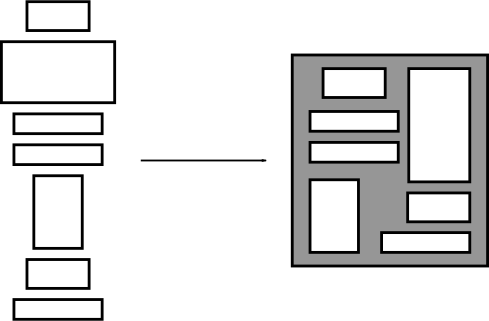
\includegraphics[width=.5\textwidth]{problem}
\caption{An example of the problem and the graphical solution}
\label{fig:problem}
\end{figure}

\begin{figure}
\centering
\subfloat[assignement]{
\begin{minipage}{.45\textwidth}
\centering
module {\tt A} $= 10 \times 20$ \\
module {\tt B} $= 20 \times 50$ \\
module {\tt C} $= 10 \times 50$ \\
module {\tt D} $= 30 \times 20$ \\
\end{minipage}
} \hfill
\subfloat[solution]{
\begin{minipage}{.45\textwidth}
\centering
place module {\tt A} at $(0, 0)$ \\
place module {\tt B} at $(10, 0)$ \\
place module {\tt C} at $(0, 20)$ \\
place module {\tt D} at $(10, 50)$ \\
\end{minipage}
} \\
\caption{Example problem assignment and the solution as the text}
\label{fig:sample}
\end{figure}

\section{Problem Coding}

During the last decade, several different representations were introduced. They differ in the set of floorplans they can encode and in the complexity of the encoding/decoding algorithm. For example, some representations are very compact in size and fast in decoding, but they can represent only a small subset of all possible floorplans.

Usually, we divide floorplans into two categories: The {\em slicing} and {\em non-slicing} floorplans. The slicing floorplans can be represented by a tree, which specifies how the individual modules are put together recursively by binary operations (bottom-up view) or how the final floorplan can be cut down to individual modules (top-down view). The non-slicing floorplans do not have such a property and they are considered as more general and versatile.

The best known slicing floorplan representation is the Polish Expression (PE) \cite{pe} that works with slicing trees. They are very simple to understand and they are convenient, but they may not comprise the optimal solution. Some examples are shown in Fig.~\ref{fig:slicing}. Non-slicing represantitions include a TCG \cite{tcg}, an integrated TCG with a packing sequence (TCG-S) \cite{tcgs}, an O-Tree \cite{otree}, a B*-Tree \cite{btree}, a Corner Block List (CBL) \cite{cbl}, a Sequence Pair (SP) \cite{sp}, and a Bounded Slicing Grid (BSG) \cite{bsg}. Some of the representations listed here are described in more details in the following chapters.

\subsection{Slicing Representation}

\subsubsection{Slicing Tree}

A tree in the area of computer science is a special type of graph used to represent hierarchical structures. Each node in a tree represents an element, and each edge represents the relation `is child of' or `is parent of'. Trees can be also used to represent floorplans that are hierarchical. The best known tree-based representation in floorplanning is probably the {\em slicing tree} written as in {\em postfix expression}.

A slicing tree is a binary tree, where each node has either zero or two descendants (children). Each node represents a certain part of the final floorplan, the so called {\em slice}. Smaller slices can be composed to create bigger slices by using certain binary operations, for example, the {\em vertical join $\oplus$} and the {\em horizontal join $\ominus$}. Each leaf node represents a module to be placed. Each internal node represents a binary operation that puts the slices represented by their children together. And finally, the root of the tree is the biggest slice representing the final floorplan. Some examples are given in Fig.~\ref{fig:slicing}.

The slicing tree is usually encoded as a postfix expression (also known as Polish notation). The postfix expression may be obtained from the slicing tree by its traversion in a post-order (see Fig.~\ref{fig:postorder}). The postfix expression does not need any brackets to retain parenthesis, the associativity is maintained by the positions of the symbols. 

\begin{figure}
\centering
\begin{algorithmic}[1]
  \STATE{traverse left subtree (if any) of current node $ N $ using this function}
  \STATE{traverse right subtree (if any) of current node $ N $ using this function}
  \PRINT{the current node $ N $}
\end{algorithmic}
\caption{The post-order traversion pseudocode}
\label{fig:postorder}
\end{figure}

This representation has many pros and cons. It is very easy to implement because of the recursion contained, the number of the nodes in the tree does not change during the computation, and the search space is small. However, only the slicing floorplans are considered. In case that the optimal floorplan is not slicing, it cannot be found using this representation.

The search space of the slicing tree representation \cite{otree} has the size equal to $O(n!2^{5n-3}/n^{1.5})$. Each floorplan can be encoded using $n(6+\lceil\log n\rceil)$ bits.

However, in the 2001 article by M.~Lai and D.F.~Wong \cite{pe2}, it was proven that by using the slicing tree representation and compaction, all maximally compact placements of modules can be generated. Therefore, under certain conditions, the slicing tree can be considered as a representation for all non-slicing floorplans as well.

\begin{figure}
  \centering
  \subfloat[floorplan 1]{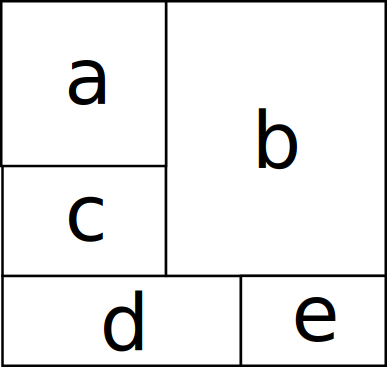
\includegraphics[height=4cm]{slicing1f}} \hspace{1cm}
  \subfloat[slicing tree 1]{\includegraphics[height=4cm]{slicing1t}} \\
  \subfloat[floorplan 2]{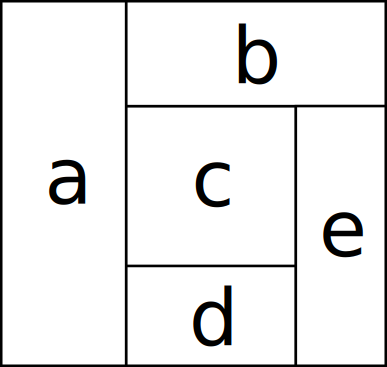
\includegraphics[height=4cm]{slicing2f}} \hspace{1cm}
  \subfloat[slicing tree 2]{\includegraphics[height=4cm]{slicing2t}} \\
  \caption{An example of slicing floorplans and their trees}
  \label{fig:slicing}
\end{figure}

\subsection{Non-Slicing Representations}

\subsubsection{Sequence Pairs}

The sequence pair representation encodes the geometric relations of modules instead of encoding the floorplan structure itself. Let us have a set $M$ of modules. A sequence pair of module set $M$ is a pair of sequences of distinct names of all modules from $M$. For example, for $M = \{a,b,c\}$, the tuple $S = (\mathrm{acb},\mathrm{bac})$ is a valid sequence pair. Each sequence pair specifies the module placement topology by a group of rules, called the {\em horizontal (vertical) constraints}:

$$ S = (\cdots \circ \cdots \bullet \cdots, \cdots \circ \cdots \bullet \cdots) \rightarrow x_\circ + w_\circ \leq x_\bullet $$
$$ S = (\cdots \bullet \cdots \circ \cdots, \cdots \circ \cdots \bullet \cdots) \rightarrow y_\circ + h_\circ \leq y_\bullet $$

A sequence pair is said to be {\em feasible} if there is a feasible packing which satisfies the constraints. Otherwise, it is called {\em infeasible}. It is proven \cite{nphard} that all the sequence pairs for unpositioned modules of fixed size are feasible. An example of a floorplan encoded by the sequence pair is shown in Fig.~\ref{fig:sp}. As we can see from the grid, when the node labels are read left to right, they form the sequence {\tt fcbead}. If they are read top to bottom, they form {\tt ecadfb}.

The search space of the sequence pair representation \cite{otree} has the size equal to $O((n!)^2)$. Each floorplan can be encoded using $2n(\lceil\log n\rceil)$ bits. The solution space always contains the optimal solution, if there is any.

\begin{figure}
\centering
\subfloat[floorplan]{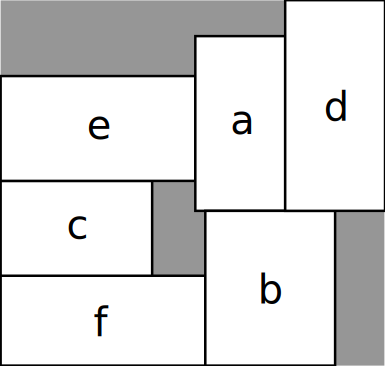
\includegraphics[width=0.45\textwidth]{spf}} \hfill
\subfloat[sequence pair constraints]{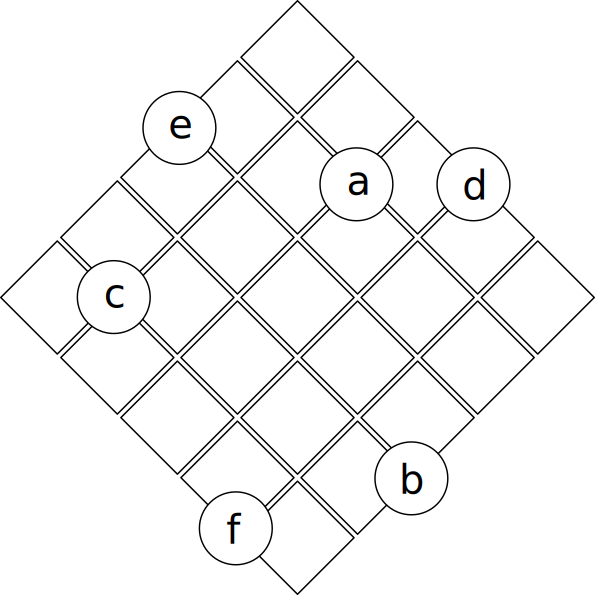
\includegraphics[width=0.45\textwidth]{sp}}
\caption{Example floorplan encoded by a sequence pair $(\mathrm{ecadfb}, \mathrm{fcbead})$}
\label{fig:sp}
\end{figure}

\subsubsection{O-Tree}

The O-Tree representation \cite{otree} can be used in order to represent non-slicing floorplans. The placement can be obtained from an O-Tree in amortized linear time to a number of modules, providing that a special {\em contour} cache structure is used.

An O-Tree is a rooted directed tree in which the order of the subtrees is important. Each O-Tree can be encoded as a tuple $(T, \pi)$, where the $T$ is a bit string of length $2(n-1)$ representing the tree branching structure (0 = step on descending edge, 1 = step on ascending edge) and the $\pi$ is a permutation of modules used for the tree node labeling. The first element in $\pi$ is the tree root. An example of a floorplan encoded by an O-Tree is shown in Fig.~\ref{fig:otree}.

A floorplan is {\em L-compact} if and only if no module can be shifted left without overlapping other modules. A floorplan is {\em B-compact} if and only if no module can be shifted down without overlapping other modules. A floorplan is {\em LB-compact} if and only if it is L-compact and B-compact. A floorplan is {\em admissible} if it is LB-compact. An O-Tree is admissible if the corresponding floorplan is admissible.

Given any placement, there is corresponding LB-compact placement that can be created by a sequence of $x$ direction and $y$ direction compactions. The total area of the resulting LB-compact placement is less or equal to the area of the original placement.  

There is a one to one correspondence between an admissible floorplan and its O-Tree representation.

The search space of an O-Tree representation \cite{otree} has a size of $O(n!2^{2n-2}/n^{1.5})$ (while searching for admissible floorplans only). Each floorplan can be encoded using $n(2+\lceil\log n\rceil)$ bits. The solution space always contains the optimal solution, if any.

\begin{figure}
\centering
\subfloat[floorplan]{\includegraphics[width=0.45\textwidth]{otreef}} \hfill
\subfloat[O-Tree]{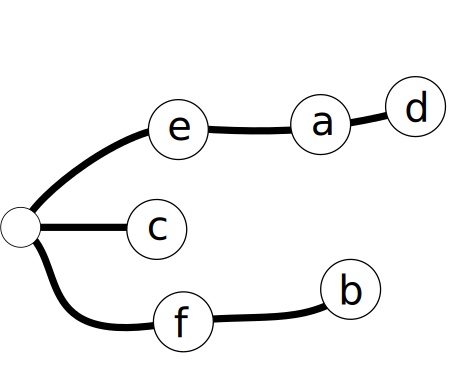
\includegraphics[width=0.45\textwidth]{otree}}
\caption{An example floorplan encoded by an O-Tree $(\mathrm{001101000111}, \mathrm{fbcead})$}
\label{fig:otree}
\end{figure}

\begin{figure}
\centering
\subfloat[whole contour]{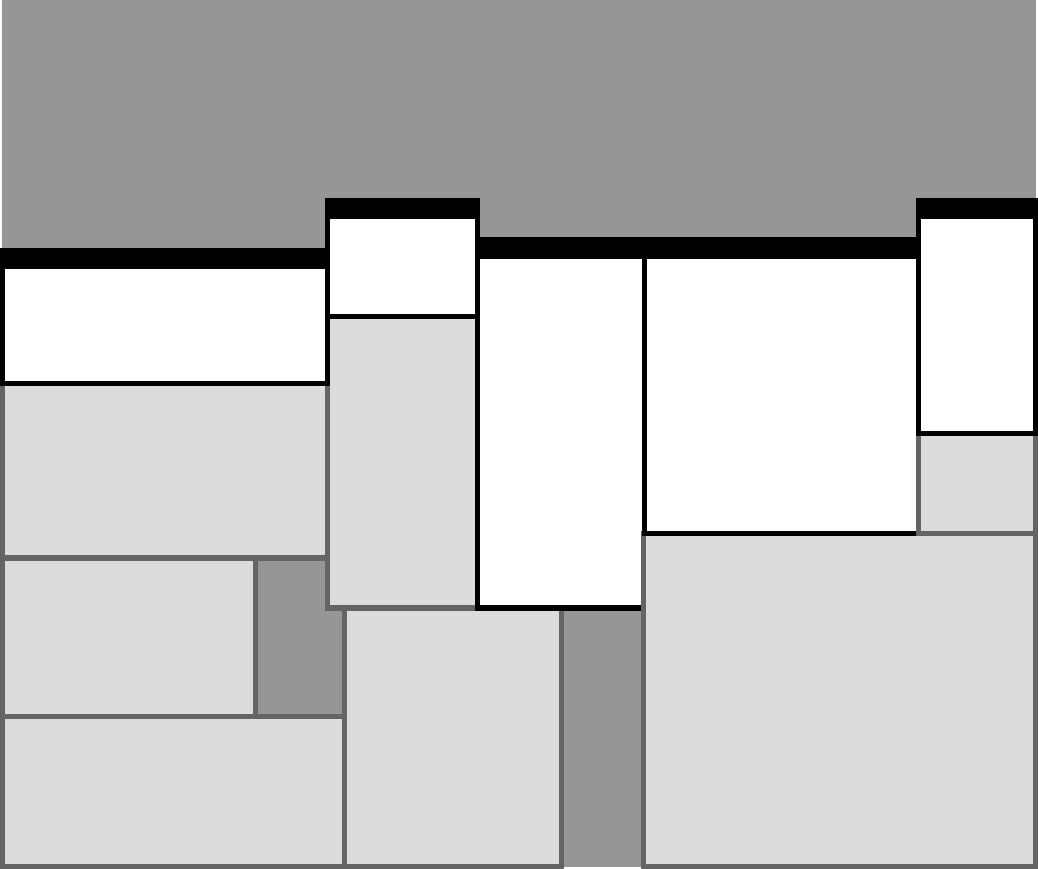
\includegraphics[width=0.45\textwidth]{contour1}} \hfill
\subfloat[contour part evaluated]{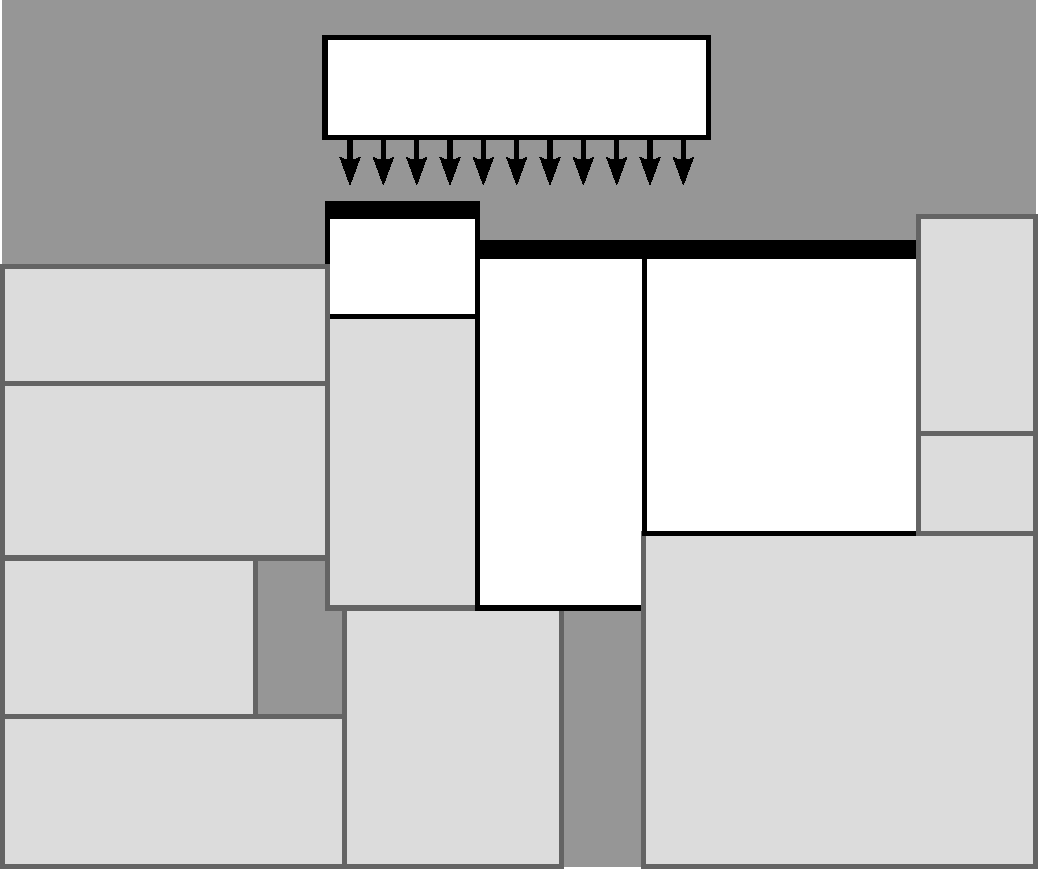
\includegraphics[width=0.45\textwidth]{contour2}}
\caption{The contour structure and its application}
\label{fig:contour}
\end{figure}

\subsubsection{B*-Tree}

The B*-Tree representation \cite{btree} is closely related to the O-Tree representation. It is also based on a tree (binary tree) and uses the similar placement algorithm. In addition, the representation has asymptotically the same number of combinations ($O(n!2^{2n-2}/n^{1.5})$) and uses the same terminology relating the admissible and not admissible floorplans.

The big advantage of the B*-Tree representation is that it is quite simple to add support for general rectilinear modules (encoded as fixed subtrees) or pre-placed modules (nodes in the B*-Tree with position fixed), even soft modules. Furthermore, B*-Tree evaluation can be done incrementally by evaluating the updated subtree only.

The B*-Tree \cite{btree} structure keeps the geometrical relationship between modules as follows. The root is located at $(0, 0)$. If the node $b$ is the left child of the node $a$, the module must be located on the right-hand side and adjacent to the module $a$, that is $x_b = x_a + w_a$. If the node $c$ is the right child of the node $a$, the module must be located above and adjacent to the node $a$, that is $x_c = x_a$. The $y$ coordinate depends on already placed nodes and must be computed as the top-most point of already placed modules that lie under the module newly placed. A special helper contour structure is used in order to speedup this searching.

\begin{figure}
\centering
\subfloat[floorplan]{\includegraphics[width=0.45\textwidth]{btreef}} \hfill
\subfloat[B*-Tree]{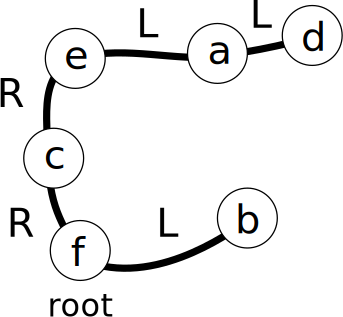
\includegraphics[width=0.45\textwidth]{btree}}
\caption{Example floorplan encoded by a B*-Tree}
\label{fig:btree}
\end{figure}

\chapter{Suggested Approach}
\label{sec:approach}

In this chapter, a new approach for solving the floorplanning problem is introduced and described in more details.

\section{B*-Tree}

Coding is a crucial part of every evolutionary algorithm. It influences the size and the characteristic of the search space, the quality of the solution and the speed of coding and decoding. As the decoding is executed for every iteration, generation and individual, its speed is critical. For example, if we use 1,000 iterations, 500 generations and have population of 100, the coding process may be executed $ 1000 \cdot 500 \cdot 100 = 50,000,000 $ times. If the decoding process takes 1 ms, the total time of 13 hours is reached. Of course, this count can be lowered by evaluating only individuals not already evaluated. But still the coding takes a large amount from the algorithm running time.

Therefore, the B*-Tree representation \cite{btree} was chosen to be used in the suggested algorithm. The B*-Tree is a regular hierarchical structure, allowing effective tree operations (including placing) and providing many options for tree permutation. By altering the B*-Tree nodes, many different floorplans can be created from the original prototype easily. 

As noted in previous chapters, the conversion from the B*-Tree to the placement can be done in amortised linear time using the {\em contour data structure} (or similar), introduced in \cite{otree}. Without this structure, the worst case would be quadratic to the number of modules.

B*-Tree does not differ from the ordinary binary tree, a common data structure, often used in many implementations of sets, priority queues, etc. The only difference is in values it holds. The algorithm will work with B*-Trees of modules, both unplaced and placed.

Also, for doing permutations using the POEMS actions, all B*-Tree nodes must be addressable. So each node in a B*-Tree gets an unique integer number, which is used as its address. Further, for creating new or random POEMS actions, it will be also required to generate random addresses. As an each address is an integer, minimum and maximum values must be known at the creation time. Minimum value is defined as $0$, maximum value as $n-1$, where $n$ is a number of modules in the problem set. To make this solution more generic, a counter class is introduced. It allows tree to be numbered by a `hot potato' algorithm and then the last number used can be easily extracted from the same counter object.

Some examples of B*-Tree encoded floorplans are shown in Fig.~\ref{fig:btreef} and Fig.~\ref{fig:btrees}.

\begin{figure}
\centering
\includegraphics[width=.8\textwidth]{btreebig1}
\caption{An example of a floorplan represented by the B*-Tree}
\label{fig:btreef}
\end{figure}

\begin{figure}
\centering
\includegraphics[height=.8\textheight]{btreestruct}
\caption{An example of a floorplan structure represented by the B*-Tree}
\label{fig:btrees}
\end{figure}

\subsection{Placement}

Placement is an assignment of an exact 2D position to each module. In other words, it is a conversion from the B*-Tree of unplaced modules to the B*-Tree of placed modules, which can be done recursively. The root is placed at $(0, 0)$. Then the recursive procedure starts. First, the left subtree of the current node is placed, then the right one.  

When placing the node $i$, the position of its parent $(x_p, y_p)$ is already known. If the node visited is the left child of the parent, its position is defined as $(x_p+w_p, y_i)$, where $y_i$ is the maximal $y$ coordinate of already placed modules which overlap the horizontal interval $(x_p+w_p, x_p+w_p+w_i)$ (quickly obtained by the contour structure). 

If the node visited is the right child of the parent, its position is defined as $(x_p, y_i)$, where $y_i$ is the maximal $y$ coordinate of already placed modules which overlap the horizontal interval $(x_p, x_p+w_i)$ (quickly obtained by the contour structure). 

The helper structure for finding the overlapping modules used in the proposed algorithm (similar to the contour structure) is described in the next chapter.

\subsubsection{Contour helper structure}

The contour structure is used in both \cite{otree} and \cite{btree} to speedup the searching for an $y$ coordinate of the newly- placed module (the other $x$ coordinate is simply given by its parent node). Without this structure, searching would have complexity of $O(n^2)$, where $n$ is the number of modules. It is because all already placed modules must be checked for overlap before placing each module. 

The original contour structure \cite{otree} holds only a subset of already placed modules, which form the `skyline' of the placement. Only these modules must be searched to find the $y$ coordinate of the newly placed module. Usage of the structure is shown in Fig.~\ref{fig:contour}.

In this work, a similar approach is used. Instead of using a doubly linked list of placed modules, the priority queue was used. In this queue, modules are sorted by their top-most $y$ coordinate (descending). Before placing each module, the queue is walked starting from the head until the first module is reached that overlaps with the module being placed. The top-most $y$ coordinate of the module found in the queue is then used as an $y$ coordinate of the newly placed module.

The complexity of this approach should be similar to the original algorithm widely used, it is easier to implement and less error-prone. The performance of the resulting algorithm is evaluated in Table~\ref{tab:placer}.

\section{Evolutionary Algorithms}

\cite{vh} Looking into the world of nature, we can see that a huge number of very difficult problems have been solved since the beginning of the world‘s existence. It was, for example, parts of the body and organs, and their functions in the body. Living creatures have had to learn how to survive in dangerous and changing enviroment. Searching for food, escaping from agressors, raising young ones\ldots these are just several examples of what living beings face and have to solve every day. Life in its richness, all around us, is an evidence that these problems have been and are solved successfully.

It is widely known that the life is based on genetic information (RNA, DNA) and - since the very beginning, the genetic information is being slowly but continuously modified by e.g. radiation or other random physical processes. If a creature whose genetic information was modified grows adult, it can reproduce, preserve and pass their genetic information onto the next generation. In addition, individuals can combine their genomes: hence, higher quality may be created by means of hybridization (crossover). This process, in a long prospective, is called and described as {\em evolution}.

The mankind is an integral part of the nature, and draws inspiration from the nature every day - in music, art, construction, and in problem-solving as well. Using modern computer technology, it is possible to simulate the ways in which the nature faces various challenges and use them for solving real world problems.

The scientific branch that deals with research in natural ways of problem-solving and simulates these processes with use of computers is called {\em soft-computing}. This branch has existed for decades and it has already influenced various areas of computer technology and cybernetics. Because of continuous development and progress in this field, we can use and enjoy numerous achievements of modern technology. The already mentioned simulated evolutionary processes are called {\em evolutionary algorithms} - as they, in fact, may simulate the evolution. The main purpose of them is a search for an optimal solution for a particular problem.

The subject-matter of this work is the application of the {\em POEMS} iterative optimisation framework \cite{poems} and the {\em genetic algorithm} to the 2D rectangle packing problem (also known as {\em floorplanning}). This optimisation problem is NP-hard and suitable for evolutionary algorithms.

Evolutionary algorithms are inspired by on evolutionary processes in the nature. They are popular and widespread, as they are easily grasped even by novice researchers and programmers, but they do not guarantee good results in all scenarios automatically. The key \cite{hynek} is to use as much knowledge about the concrete problem as possible or combine the evolutionary algorithms with the traditional approaches (the process is called {\em hybridization}).

\subsection{Advantages}

\begin{itemize}
\item{The algorithms may be customized in order to solve a difficult problem without even knowing its semantics. This is useful for NP-complete problems where no efficient algorithm is known or does not exist at all.}
\item{Acceptable solutions are usually found in reasonable time.}
\item{Most of the processes may be easily implemented and may be run efficiently on parallel computers. This leads to performance scalability.}
\item{They are generally easy to understand because they simulate natural processes.}
\end{itemize}

\subsection{Disadvantages}

\begin{itemize}
\item{These algorithms are not exact: therefore, they are not usable for critical applications. One cannot guarantee that the evolutionary algorithm will find the best solution every time the algorithm is started.}
\item{They work mostly on a random basis. Hence, they may produce different results after every execution.}
\item{Sometimes they `get stuck' at a certain sub-optimal solution, and further improvement is hardly found. Nevertheless, computer scientists often come up with evolutionary algorithm modifications that can slow the `get-stuck process' down or even eliminate it.}
\item{Evolutionary algorithms cannot be used as a universal and `magic' method for solving of all problems in the world. Some voices say that the increasing popularity of evolutionary algorithms is for bad - they are afraid that new computer scientists will lose interest in traditional algorithm research.}
\end{itemize}

\subsection{Basic Types}

\begin{itemize}
\item{{\em Genetic Algorithms} are well-known and versatile evolutionary algorithms. They are based on genetics-related ideas. There is a population of individuals and each of them carries one candidate solution encoded in their genomes. In addition, there is an objective quality-measuring function, the fitness function. It expresses how `good' the solution is. The algorithm runs in iterations that are called `generations'. In every generation, a new population is created by selecting best individuals in the old population and combining them. The algorithm iterates until its terminal condition is encountered, and then returns the best individual found as the problem solution. This algorithm is described in more details below.}
\item{{\em Genetic Programming} uses modified genetic algorithms in order to optimise and generate programmes (instead of encoded solutions). A genetic program comprises a tree structure. It is optimised by adding, removing or moving its tree nodes.}
\item{{\em Memetic Algorithm} is a hybrid genetic algorithm, based on memes instead of genes. Unlike genes, mems can adapt themselves over time.}
\item{{\em Cultural Algorithm} is similar to the genetic algorithm: contrary to it, a cultural algorithm contains a knowledge component - population is enriched by a set of `beliefs', that are shared, used and extended by all individuals. Therefore, it is more similar to the real society.}
\end{itemize}

\section{Genetic Algorithm}

The genetic algorithm is one of the best-known evolutionary algorithms. It was first introduced and researched by John Holland \cite{ga}. The method is inspired by Darwin's theory of evolution \cite{darwin} that describes the development of the life as a continuous struggle between living beings and their enviroment. Only the individuals of highest quality are able to adapt to the natural enviroment - hence survive and reproduce. We can simulate the process in the computer, using problems as an enviroment, and their candidate solutions as individuals.

The very first task for a genetic algorithm designer is to find effective coding of the problem solution. Such coding is to maintain all characteristics of each solution and should be simply creeditable by mutation and crossover operators. For a proper function of the algorithm, a good coding is crucial. For optimisation problems, where both feasible (acceptable) and infeasible (unacceptable) solutions are considered, some kind of additional repair operation may be required to convert an infeasible solution to a feasible one.

What we need is an objective quality-measuring function that will tell us how good the particular solutions are. In nature, this function is simply the ability of individual to survive and reproduce. In an evolutionary algorithm, the function is called {\em fitness function}. This function takes the encoded candidate solution as a parameter, and returns a numeric value. This function should return the maximal (or minimal) value for the optimal solution only (providing that it exists).

To simulate the evolution, genetic algorithms work in iterations that are called {\em generations}. First, an initial population is generated. In every following generation, new individuals are created from the current population with use of {\em selection}, {\em crossover} and {\em mutation} operators. These operators come from their real world counterparts.

New individuals are either copied into a new empty population (generational model, Fig.~\ref{fig:ga_pseudocode_dynamic}) or they replace the worst solutions in the current population (steady-state model, see Fig.~\ref{fig:ga_pseudocode_static}).

To summarise the chapter, before the genetic algorithm can be used for solving a problem, we need to specify the following: the effective coding of the solution; the fitness function; the algorithm for creating the initial population; the selection operator(s); the mutation operator(s); the crossover operator(s); and we have to select the algorithm parameters (but they are usually decided at the run time).

\begin{figure}
\centering
\begin{algorithmic}[1]
  \STATE{create an initial population $ P_0 $ (usually random)}
  \STATE{evaluate the fitness of each invidivual in $ P_0 $}
  \FOR{$ g $ in range 1 .. $ g_{max} $}
    \STATE{create a new empty population $ P_g $}
    \STATE{take individuals from $ P_{g - 1} $ using the selection operator and copy them into the new population $ P_g $ either directly or using crossover and mutation operators}
    \STATE{evaluate the fitness of each individual in $ P_g $}
    \STATE{replace the old population $ P_{g - 1} $ by the new population $ P_g $}
  \ENDFOR
  \RETURN{best-ranked individual from $ P_g $}
\end{algorithmic}
\caption{Genetic algorithm pseudocode (generational model)}
\label{fig:ga_pseudocode_dynamic}
\end{figure}

\begin{figure}
\centering
\begin{algorithmic}[1]
  \STATE{create an initial population $ P $ (usually random)}
  \STATE{evaluate fitness of each invidivual in $ P $}
  \FOR{$ g $ in range 1 .. $ g_{max} $}
    \STATE{take individual(s) from $ P $ using selection operator, apply crossover and/or mutation operators, and replace worst individuals in population $ P $ by them}
    \STATE{evaluate fitness of each individual in $ P $}
  \ENDFOR
  \RETURN{best-ranked individual from $ P_g $}
\end{algorithmic}
\caption{The genetic algorithm pseudocode (steady-state model).}
\label{fig:ga_pseudocode_static}
\end{figure}

\subsection{Initial Population}

Every run of a genetic algorithm begins with a creation of an initial population. It is convenient to generate random solutions in order to cover the widest area within the searching space as possible. We can achieve better results or better performance if we generate additional initial solutions in the areas in which we expect the optimal solution to be found.

There is an important parameter of the genetic algorithm, the {\em population size}. If the population size is too low, the algorithm may degenerate, and nothing new will be found. On the other hand, an excessive population may slow the algorithm down and cause that the algorithm is of no use. There is nothing like a universal value: anyway, in most cases, 50--1000 individuals would be enough.

Some implementations use a special operation, called `immigration'. The immigration causes that some parts of the current population can be replaced by new individuals, either random or created by another (parallel) genetic algorithm. Parallel genetic algorithms are called `population islands', to resemble the reality of several isolated populations. The exchange of individuals between these islands can increases the population diversity.

\subsection{Solution Coding}

The solution coding is the way how the solutions are represented in individual's chromosome. This is probably the most important part of a genetic algorithm. A single problem may be encoded in various ways, and efficient coding is the key to its successful solution. When a genetic algorithm fails, the mistake often is the coding. One coding frequently used is the binary string encoding or the tree encoding.

Binary string encoding is often used for numbers or array of numbers. Numbers are mostly not represented directly, but in a better suited coding, such is the Gray code. If a bit changes in Gray code (e.g. by a mutation operator), the number it represents alters only a little. In a direct representation, MSB flip means much bigger change than flipping LSB. On the other hand, trees represent expressions or computer programs (e.g. in genetic programming, see~\cite{koza}), or other recursive structures. Trees are often encoded as strings using prefix of postfix coding, as i t does not need brackets to retain parenthesis.

\subsection{Fitness Function}

The fitness function, which may be defined for every chromosome, is used for evaluation of the solution quality. The function usually returns non-negative real values: the greater the value is, the better the solution, so the best solution is simply the one with the greatest fitness value. The purpose of the genetic algorithm is to find a solution with the greatest fitness value possible using available operators and in the given time or resource contraints.

There is a simple way to include more parameters in the fitness function: the form $ f(s) = \sum_{\forall i} w_i \cdot X_i \; \; (\sum_{\forall i} |w_i| = 1, |w_i| \in \langle 0,1 \rangle) $, where $ w_i $ is a real number expressing `importance' or `weight' of the input parameter $ X_i $. If we set zero as the weight, the parameter will not be optimised. Alternatively, we can set negative numbers as the weight, if we want to minimise the parameter value.

\subsection{Selection Operator}

In every generation, we can either select certain number of couples and create offsprings by means of crossover operators, or just select sufficient amount of some individuals to clone themselves into a new generation. If we really want to simulate evolution, we must prefer `better' solutions over `worse' ones. That is, the individuals with greater value of the fitness function. There are many ways to accomplish that selection and they are called {\em selection operators}. Some kinds of selection operators are described below.

\subsubsection{Roulette Selection}

Roulette selection is one of the most common algorithms for selection. Every individual is selected with probability according to its relative fitness. There are more variants of the algorithm, because the basic one fails in certain scenarios. The algorithm is based on cumulative fitness and a random threshold that must be satisfied.

\subsubsection{Tournament Selection}

Another simple and widely used type of selection operator is the tournament selection. This algorithm is inspired by struggle between two or more animals for survival. It is obvious, that the `better' animal with higher fitness defeats its enemy, survives and can reproduce itself into another generation. In \cite{tournament} an improvement is suggested, that the better individual should not win always, but only in cca 95\% cases. General algorithm description can be found on Fig.~\ref{fig:tournament}.

\begin{figure}
\centering
\begin{algorithmic}[1]
  \STATE{take $ N $ random individuals from the population}
  \IF{random real number $ \in \langle 0, 1) < 0.95 $}
    \RETURN{individual with the best fitness}
  \ELSE
    \RETURN{random individual}
  \ENDIF
\end{algorithmic}
\caption{The tournament selection algorithm pseudocode}
\label{fig:tournament}
\end{figure}

\subsubsection{Elitism}

There is another good idea in genetics algorithms, the {\em elitism}. The $ N $ best ranked individuals are always copied into the new generation as they are, without any change at all. It prevents the best solution from disappearing from the population.

\subsection{Crossover Operator}

The crossover operator is used in order to combine two or more individuals to produce a new, desirably better ones. The means of the combination may be very simple, for example, splitting parents and then mixing the parts together to create two hybrid descendants. The aim of the crossover is to select best features from both parents, and retain their good attributes into the following generation with the chance of creating even better genome when combining ones. Normally, we do not know which part of parent is the best - so we simply let the crossover happen with certain probability and see if the offspring survives over time. Nevertheless, even `bad‘ descendants may contribute in the process of the search for the optimal solution - since they increase the population diversity. An example of a crossover process is shown in Fig.~\ref{fig:crossover}.

\begin{figure}
\begin{center}
$ \Box \Box \Box \Box \Box \Box \; + \; \blacksquare \blacksquare \blacksquare \blacksquare \blacksquare \blacksquare \; \rightarrow \; \Box \blacksquare \blacksquare \Box \Box \blacksquare $
\end{center}
\caption{The crossover in genetic algorithm}
\label{fig:crossover}
\end{figure}

\subsection{Mutation operators}

The mutation is usually a slight change in individual genetic information. It is caused mainly by radiation or other random physical or chemical processes. The mutation is an engine of the evolution because it often finds an unexpected improvement of current solutions. On the other hand, the mutation may be harmful because it may damage a good individual, too. Some experts say that the mutation is a key part of the genetic algorithm while other operators are only tools for spreading good changes found by mutation through the whole population. An example of the mutation is shown in Fig.~\ref{fig:mutation}.

\begin{figure}
\begin{center}
$ \Box \blacksquare \Box \Box \blacksquare \Box \; \rightarrow \; \Box \blacksquare \blacksquare \Box \blacksquare \Box $
\end{center}
\caption{The mutation in the genetic algorithm}
\label{fig:mutation}
\end{figure}

\section{POEMS Algorithm}

A standard genetic algorithm works directly with solutions yet the POEMS approach introduced in \cite{poems} in combination with the genetic algorithm rather evolves solution modifications. This is a promising method that may prevent (in certains situations) the genetic algorithm from getting stuck at a sub-optimal solution.

The POEMS method works in iterations. Before the first iteration, an initial solution is generated. This solution is called a {\em prototype}. The aim of the following iterations of the POEMS algorithm is to find the best modification of the prototype with use of the genetic algorithm, which serves as a modification optimiser. The prototype modifications are obtained by applying {\em sequences} of defined {\em actions} onto the prototype solution. After each iteration, if an improvement is found, the prototype is replaced. 

In every iteration, a steady-state genetic algorithm is executed in order to find the optimal action sequence. First, a population of $N$ random action sequences of length $L$ is created. The sequences are composed of individual actions and their parameters. The evolution is started, and a selection, crossover and mutation operators are used in order to breed the action sequences. The fitness function of each action sequence is defined as a fitness of the prototype solution after being modified by the particular sequence evaluated.

Generally speaking, POEMS is an iterative stochastic algorithm which uses the genetic algorithm (or some other evolutionary algorithm) for doing the local search during each iteration.

\subsection{Prototype}

A prototype is the initial solution created and improved by the POEMS algorithm. Its creation is a very important step, because the initial position highly influences the space searched. As the solutions are binary trees, a way of creating trees from the initial set of modules must be introduced. 

Two ways of prototype creation were introduced - {\em complete tree} heuristic and {\em best-fit} heuristic. For producing significantly better results, the best-fit heuristic was used in final benchmarks.

\begin{figure}
\centering
\subfloat[complete tree]{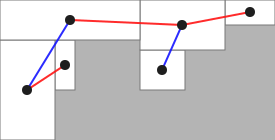
\includegraphics[height=4.5cm]{prototype1}} \hspace{1em}
\subfloat[best-fit heuristic]{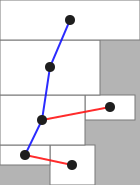
\includegraphics[height=4.5cm]{prototype2}}
\caption{Two ways of creating a prototype example}
\label{fig:prototype}
\end{figure}

\subsubsection{Complete tree heuristic}

The aim of the complete-tree prototype generator is to create a tree as similar to the complete tree as possible. All nodes, except the ones in the last floor, must have exactly two children and must be balanced. 

First, an array of modules is created. The modules are preprocessed by rotation so they are wider than higher. After the rotation, they are sorted by width descending (descending) and height (ascending). Then, the algorithm for creating a heap from an array is used for generating the complete tree from this array of sorted modules.

\subsubsection{Best-fit heuristic}

The best-fit heuristic is a general name for a greedy rectangle packing algorithm. The principle is to select the best fitted module for each hole in the final placement. Both holes and modules are stored in a queue and the algorithm iterates until the module queue is empty. After each placement of the module, the whole list is updated.

A simple heuristic inspired by the best-fit heuristic was introduced to produce accurate prototypes in the suggested floorplan solver. First, it rotates all modules so they are wider than higher and sorts them by width (descending) and height (ascending). This array represents a queue of the modules. 

Then, the tree is built level by level. On each level, a certain limited horizontal space must be filled. Initially, the space to be filled equals to the width of the widest rectangle or the square root of all modules area, whichever is bigger (this is further referred as the {\em original value}). Until the module queue is empty, the algorithm selects the first module from the queue, which can be placed into the space. Then, the module is removed from the queue and the space is shortened by its width. If there is no such module small enough to fit into the space, the current level is ended and a new level is started with the space reset to the original value. 

During this procedure, a tree is being built. The first module placed is marked as the B*-Tree root. The next module in the same level is placed as the left subtree of the previous module and the first module on the next level as the right subtree of the first module in the current level.

\subsection{Actions}

Each action in the POEMS algorithm \cite{poems} represents a certain parameterised modification of the prototype. Individual actions are joined together to sequences that are optimised by the genetic algorithm. 

Every action has a Boolean flag that {\em enables} or {\em disables} the action. If the action is disabled, it does nothing to the input tree. Disabled actions can be used as a special kind of placeholder. \footnote{Disabled actions are somewhere reffered as {\em NOP actions} and enabled actions as {\em active actions}.}

If the enabled and disabled actions were treated equally, the population would be soon infested by disabled actions, because doing nothing to the prototype results in usually better fitness than modifying it somehow. This is the reason for introducing the so called {\em nichés} into the algorithm. Each niché $n$ is a group of individuals that contains only sequences with $n$ or more enabled actions. These nichés are used by the selection operator and during the insertion of the new individual into the population.

Now, the individual action types and their parameters will be introduced.

\subsubsection{Rotate action}

Rotate action flips and mirrors subtrees of every node in the whole subtree starting from the specified tree node. The result is similar to the rotation.

\noindent
\begin{tabular}{|l|l|}
\hline
Parameter 1 & Number of the node to start the rotation from. \\
\hline
\end{tabular}

\subsubsection{Flip action}

Flip action flips (rotates) the module of the specified tree node. If the module is already flipped, it is reverted to its original state.

\noindent
\begin{tabular}{|l|l|}
\hline
Parameter 1 & The number of the node to flip. \\
\hline
Parameter 2 & The action is recursive. \\
\hline
\end{tabular}

\subsubsection{Mirror action}

A mirror action changes the left and the right child of the specified tree node. This action does nothing on the leaf node.

\noindent
\begin{tabular}{|l|l|}
\hline
Parameter 1 & The number of the node whose children will be swapped. \\
\hline
Parameter 2 & The action is recursive. \\
\hline
\end{tabular}

\subsubsection{Exchange value action}

An exchange value action takes two specified nodes and swaps their values. The tree structure is not changed, only the shape of resulting placement is different.

\noindent
\begin{tabular}{|l|l|}
\hline
Parameter 1 & Number of the first node to swap its value. \\
\hline
Parameter 2 & Number of the second node to swap its value. \\
\hline
\end{tabular}

\subsubsection{Exchange node action}

The exchange node action takes the first node specified and inserts it at the position of the second node specified. The second node is placed on the original position of the first node. This operation is permitted only if the first node does not lie in the subtree of the second node and vice versa.

\noindent
\begin{tabular}{|l|l|}
\hline
Parameter 1 & Number of the first node to swap. \\
\hline
Parameter 2 & Number of the second node to swap. \\
\hline
\end{tabular}

\subsubsection{Hang node action}

A hang node action takes the specified source node and places it as the left or the right child of the target node specified. If the target node is located in the subtree starting from the source node, nothing is done. If the target node contains a child at the target position, the child is replaced by the source node and inserted at the original position of the source node.

\noindent
\begin{tabular}{|l|l|}
\hline
Parameter 1 & Number of the source node. \\
\hline
Parameter 2 & Number of the target node. \\
\hline
Parameter 3 & Side to hang on (left or right). \\
\hline
\end{tabular}

\subsection{Genetic Algorithm}

Although various optimisation algorithms can be used in POEMS, the genetic algorithm was chosen. It can be highly customized and the author has some experience with it from previous projects. The steady-state variant was used, because it reaches the convergence quicker.

\subsubsection{Individual and fitness function}

Each individual in the population represents a sequence of actions, which, if applied to the prototype floorplan, creates another floorplan. The fitness function of each individual is computed from the evaluation of the modified floorplan which is created by applying the individual's action sequence to the prototype (each individual gets a reference to the prototype). The fitness value used is the negative amount of the unused area (total area of the enclosing rectangle without the area of placed modules). The relative amount of unused area is computed as (total area $/$ used area) $-1$. Other possibilities include enclosing the rectangle perimeter, the total area or an interconnection volume, which is not considered in this work (but it can be simply added).

The fitness function is assigned the minimal value, in the case the floorplan created by the action sequence is the same as the original one (no changes were made at all). This case may arise when all actions applied cancel their changes mutually. For example, if two flip actions on the same module are done, the result is the same as if there were no flip at all. Removing the obvious useless actions causes the algorithm to search the search space more effectively, forcing it to make bigger steps.

\subsubsection{Population}

The population of the POEMS internal genetic algorithm consist of several groups, numbered from $1$ to $n$. Each group number $n$ can contain only individuals with $n$ or more enabled actions and all groups are the same size. These groups are further referred as {\em nichés}. Population should allow effective searching for individuals from a certain niché. 

\subsubsection{Genetic operators}

The selection operator used in the work is the tournament selection with 2 competitors. First, a random niché is selected. Then, two random competitors within the same niché are picked and compared. The better is returned in 95\% cases, the worse one in 5\% cases \cite{tournament}. Experiments were performed to decide if choosing individuals within the same niché produces better results than choosing both individuals randomly and the results seemed to be slightly better for the first method.

In each generation, new individuals are produced by a crossover or mutation operator (never both at the same time). The crossover algorithm is the uniform crossover, which should perform well on action sequences and is simple to implement. The mutation operator is more complex. Both small (parameter value increments, action order change) and big (parameter value randomization, action sequence shuffle) changes are made. Small changes are occuring more often than big changes. 

Each new individual produced replaces the first individual found, which is of worse or equal fitness and lower or the same niché. If no such individual is found within the population, the new individual is thrown away. This behaviour was introduced, because the algorithm tends to prefer sequences with a lot of disabled actions, as they do not `harm' the prototype. 

\begin{figure}
\centering
\begin{algorithmic}[1]
  \STATE{$n$ = random niché number}
  \STATE{take two random individuals from niché number $n$}
  \IF{random real number $ \in \langle 0, 1) < 0.95 $}
    \RETURN{individual with better fitness}
  \ELSE
    \RETURN{individual with worse fitness}
  \ENDIF
\end{algorithmic}
\caption{The used selection mechanism pseudocode}
\label{fig:tournament}
\end{figure}

\begin{figure}
\centering
\begin{algorithmic}[1]
  \STATE{$c$ = new individual with empty action sequence}
  \FOR{$ i $ in range 0 .. parent 1 sequence length $-1$}
    \IF{random real number $ \in \langle 0, 1) < 0.5 $}
      \STATE{add action at index $i$ from parent 1 to action sequence of $c$}
    \ELSE
      \STATE{add action at index $i$ from parent 2 to action sequence of $c$}
    \ENDIF
  \ENDFOR
  \RETURN{the new individual}
\end{algorithmic}
\caption{The used crossover mechanism pseudocode}
\label{fig:tournament}
\end{figure}

\chapter{Implementation}
\label{sec:implementation}

In this chapter, an implementation of the solution suggested in previous chapters is described with usage of UML class diagrams and important code fragments.

\section{Tools Used}

\subsection{Programming language}

The suggested algorithm was implemented in the Java language which is running on the official virtual machine (Oracle JVM version 1.6). The Java language was chosen mainly because of its simplicity and the rich library of collections. A lot of time and debugging was saved by using the built-in functionality, mainly collections. The most used collections include lists, sets and queues. The lists (mainly the {\tt ArrayList} implementations) are often used instead of arrays, but only at places where it is reasonable to do so. For example, an array list has a method to shuffle its elements, which can be useful in certain mutation operations.

As the Java is an interpreted language, many people are concerned about its performance. However, the speed of a well-written program coded in Java is fully comparable with the same program implemented in a low-level machine oriented language, such as {\tt C} or {\tt C++}. Advanced technologies, e.g. the JIT compilation, provide huge possibilities to optimise the bytecode by the virtual machine itself on the fly. Also, the automatic memory management in the Java Virtual Machine offers more pros than cons. Without a programmer managing the memory manually, more time can be invested to the algorithm optimisation. There is a plenty of memory these days and its reasonable usage to take advantage of caching, etc. is often more useful than saving it aimlessly.

\subsection{IDE and plugins}

All the coding was done in the Eclipse IDE (Helios). Tools used for the static code analysis, to ensure the highest code quality, include FindBugs, PMD, CodePro AnalytiX, UCDetector and ECLEmma. Unit tests were prepared using the JUnit test framework. Their code coverage is about 90\%. Most of the remaining 10\% are exceptional states or program paths that should not be reached under the normal circumstances (state checking, I/O exceptions, testing methods). The unused code was mostly deleted, but there is still some remaining in the sake of further debugging or preparing illustrations and tests for the thesis.

Code checking during the development was very strict, there are no warnings in the code (although almost all the checking rules available in the Eclipse IDE were enabled). The motivation was to use as many tools as possible to avoid technical mistakes, dodgy code, dangerous constructions and to keep the best practises through the whole codebase.

\subsection{Coding style and philosophy}

Most of the code is written using a functional approach to prevent state- related bugs and to increase the ability to write accurate unit tests. Most classes are immutable. This style allows the programmer to be less concerned about the internal state of objects. Instead of changing the object's state, a new one is created. As a drawback, more memory is used than necessary, and the garbage collector sweeps the heap more often. However, most of the objects created have a very short lifespan. Therefore, the generational garbage collector in JVM removes them quickly and reclaims a lot of memory for further use quickly.

The code contains a reasonable amount of commentaries in Javadoc. The coding style chosen is is based on C style. It features new line brackets and a lot of whitespace. There was no reason to keep up to a code guide, because the project was primarily aimed as a proof of the concept only. After all, the code formatting is the least important as the most today's IDEs feature an automatic formatter with a lot of style settings.

\section{Architecture Overview}

\begin{table}
\centering
\begin{tabular}{|p{.25\textwidth}|p{.7\textwidth}|}
\hline
{\bf Module} & Basic geometric structures (2D position, 2D rectangle, the module and the placed module). Used for decoding floorplans from their representation and evaluating the result. \\
\hline
{\bf B*-Tree} & The B*-Tree node and related utilities (the placer, the placement evaluator, the node number generator, the node number finder, the prototype generator). Used for the floorplan structure representation. \\
\hline
{\bf POEMS} & The POEMS algorithm, the POEMS actions, their sequences and the genetic algorithm for optimizing them. The heart of the floorplan problem solver. \\
\hline
{\bf Program} & Miscellaneous utilities. Used for running benchmarks, importing and exporting problems and their solutions, the logger, the utility method library and the program configuration. \\
\hline
\end{tabular}
\caption{The main program parts}
\label{tab:parts}
\end{table}

The whole program is composed of four main parts: The {\em Module} (geometry related classes), the {\em B*-Tree} (floorplan related classes), the {\em POEMS} (optimisation algorithm classes) and the {\em Program} (support classes). They are summarized in Table~\ref{tab:parts}. The suggested algorithm basically works as follows. First, the problem is loaded (for example, a benchmark) and the prototype solution is generated. Then, this prototype solution is optimised in iterations by the POEMS algorithm \cite{poems} that uses the internal genetic algorithm for local search, that is for finding the best modification of the prototype. After each iteration, the prototype is either replaced by the improvement or kept untouched as it is, whichever is better. After the specified number of iterations, the algorithm ends and outputs the improved prototype. 

The general overview schema is shown in Fig.~\ref{fig:overview} and the pseudocode in Fig.~\ref{fig:algorithm}. The individual steps will be described in more detail in the following chapters.

\begin{figure}
\centering
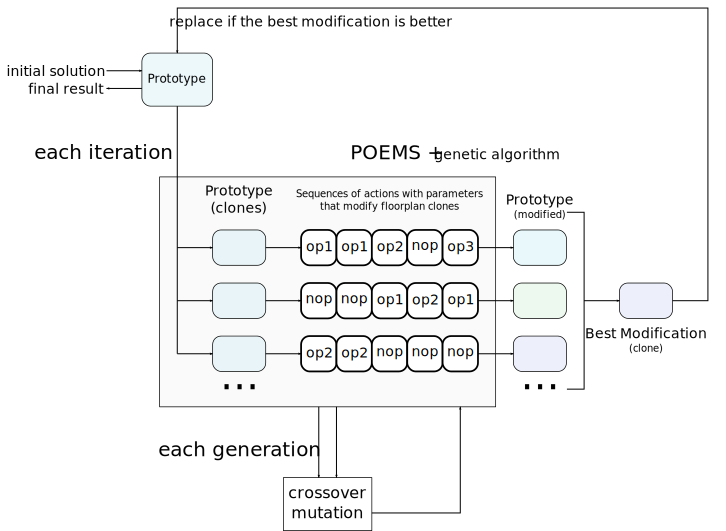
\includegraphics[width=\textwidth]{algorithm}
\caption{Overall program schema}
\label{fig:overview}
\end{figure}

\begin{figure}
\centering
\begin{algorithmic}[1]
  \STATE{create a new B*-Tree prototype $ \beta $}
  \FOR{$ i $ in range 1 .. $ i_\mathrm{max} $}
    \STATE{sequence $ S_\mathrm{best} $ = (unset)}
    \STATE{create a random population of sequences}
    \FOR{$ g $ in range 1 .. $ g_\mathrm{max} $}
      \IF{random real number $ \in \langle 0, 1) < P_\mathrm{crossover} $}
        \STATE{select two parents $ P_1, P_2 $ by applying the selection operator}
        \STATE{create two descendants $ C_1, C_2 $ using the crossover operator on $ P_1, P_2 $}
        \STATE{insert both individuals $ C_1, C_2 $ into the population}
      \ELSE
        \STATE{select one individual $ M $ by applying the selection operator}
        \STATE{create descendant $ C $ by using the mutation operator on $ M $}
        \STATE{insert the individual $ C $ into the population}
      \ENDIF
      \STATE{sequence $ S_\mathrm{temp} $ = the best sequence in the population}
      \IF{the fitness of $ S $ is better than the fitness of $ S_\mathrm{best} $}
        \STATE{$ S_\mathrm{best} = S_\mathrm{temp} $}
      \ENDIF
    \ENDFOR
    \IF{the fitness of $ S_\mathrm{best} $ is better or equal to the fitness of $ \beta $}
      \STATE{$ \beta $ = $ \beta $ modified by sequence $ S_\mathrm{best} $}
    \ENDIF
  \ENDFOR
  \RETURN{$ \beta $}
\end{algorithmic}
\caption{Overall program pseudocode}
\label{fig:algorithm}
\end{figure}

\section{Classes}

This chapter describes important classes and algorithms used in the algorithm suggested. The language in which the algorithms are presented here is not exactly the Java, but it is very similar. The main purpose of the code is to provide a low-level view on algorithms and data structures used, and any programmer should be able to understand them and re-implement them in any programming language he or she controls.

The classes are divided into the same groups, as described in the previous section. These groups are the {\em Module} (geometry related classes), the {\em B*-Tree} (floorplan related classes), the {\em POEMS} (optimisation algorithm classes) and the {\em Program} (support classes). Each group contains more Java packages, but these details are unimportant for understanding the algorithm and they are used for developer's convenience only.

\subsection{Module classes}

As the problem solved includes placing rectangles on a plane, some classes representing simple geometric objects must be created: the position is a tuple of 2D coordinates $(X, Y)$ in a 2D Cartesian space. A rectangle is defined by its width and height. The module is a named rectangle, because the name helps identify the module. The placed module is a tuple of a module and its position. 

Each module is unoriented. It means that it can be rotated freely. The rotation here means flipping the width and the height dimensions. For example, the module $A(1, 4)$ rotated is the module $A(4, 1)$. Therefore, a module must be able to rotate with its identity preserved.

The {\tt Position} class is just a tuple of two coordinates $(X, Y)$. This class is used to hold the position of a placed module. The class is immutable.

The {\tt Rectangle} class specifies the width and the height of a rectangle. The class is immutable.

The {\tt Module} class extends the {\tt Rectangle} class, adds a name, a Boolean flip flag and ability to flip the width and height. The flipping operation creates a new instance with dimensions swapped. The class is immutable.

The {\tt PlacedModule} class aggregates the {\tt Module} and the {\tt Position} classes. Each instance represents the module placed at a certain position. The class is immutable.

The class diagram of this part of the algorithm is shown in Fig.~\ref{fig:uml:module}.

\begin{figure}
\centering
\includegraphics[width=.5\textwidth,page=1]{class}
\caption{Module related classes}
\label{fig:uml:module}
\end{figure}

\subsection{B*-Tree classes}

The B*-Tree is a special kind of a binary tree. Each B*-Tree node carries a value representing exactly one module (unplaced / placed, not numbered / numbered).

The generic {\tt BTree} class represents a B*-Tree node with a value. Each node can be viewed at as a subtree, as a tree is defined recursively as a node or a parent node with child nodes. Each node instance can carry any value implementing the {\tt BTreeValue} interface. These are the {\tt Module}, the {\tt PlacedModule} and the {\tt NumberedValue}. The class is immutable.

The {\tt NumberedValue} class represents a special container for other B*-Tree value providing a tree-wide unique number for identification. This number is used as a node address in POEMS actions. The class is immutable.

The numbers are generated recursively using a {\tt Counter} class used as a `hot potato' which increments its value while visiting nodes. The last value of the counter is needed for limiting random values of POEMS actions.

The class diagram of this part of the algorithm is shown in Fig.~\ref{fig:uml:btree}.

\begin{figure}
\centering
\includegraphics[width=\textwidth,page=2]{class}
\caption{B*-Tree related classes}
\label{fig:uml:btree}
\end{figure}

\subsubsection{B*-Tree placer}

The B*-Tree {\tt Placer} class is used for assigning exact 2D position to each module based on the structure of the given B*-Tree. The rules for this placement are described in previous chapters. The important thing to mention here is, that a special structure is used here to speedup the placement. 

The speedup structure {\tt PlacerCache} is basically is a queue of instances of the {\tt PlacerCacheItem} class which are automatically sorted by their $\mathrm{level}$ property, descending. The $\mathrm{level}$ has the meaning of the top-most $y$ coordinate $\mathrm{position}$ and $\mathrm{width}$ specify the area in which the level is raised.

When placing a module, its $x$ coordinate is given by the node's parent and $y$ depends on items in the queue. The queue is walked from the beginning until a first overlapping item is reached (if none, $0$ is returned). Then, this item's $\mathrm{level}$ coordinate is used as the $y$ coordinate of the newly placed module. Finally, the queue is updated - the level is raised where the new module was placed.

As the queue is not walked whole in most situations, the speedup is significant. The placer performance is evaluated in Table~\ref{tab:placer}.

The class diagram of this part of the algorithm is shown in Fig.~\ref{fig:uml:placer}.

\begin{figure}
\centering
\includegraphics[width=\textwidth,page=3]{class}
\caption{B*-Tree placer related classes}
\label{fig:uml:placer}
\end{figure}

\subsubsection{B*-Tree evaluation}

The quality of each floorplan must be evaluated as it is used as the fitness function in the genetic algorithm. The value measured in this implementation is the amount of the unused area ($S_{\mathrm{unused}}$). For the computation of this value, the total area ($S_{\mathrm{total}}$) and the used area ($S_{\mathrm{used}}$) must be known. 

The total area of the floorplan ($S_{\mathrm{total}}$) is defined as an area of the smallest enclosing rectangle which contains all placed modules in that floorplan. The used area of the floorplan ($S_{\mathrm{used}}$) is defined as a sum of areas of all modules placed in that floorplan. 

The unused area ($S_{\mathrm{unused}}$) is then computed as the $ S_{\mathrm{total}} - S_{\mathrm{used}}$. The fitness of the floorplan is a negative value of the unused area and must be maximized (to minimize the area unused).

On the other hand, the computation of the unused area {\em percentage} ($d$) is not so clear. Various equations are used in the articles, but the most common formula seems to be $d = S_{\mathrm{total}} / S_{\mathrm{used}} - 1 $ (ratio of the unused area and the used area). The same formula is used in the proposed algorithm. An alternative formula is, for example, $d_2 = S_{\mathrm{unused}} / S_{\mathrm{total}}$.

The computation is done by the {\tt Evaluator} utility class and it is stored in an immutable instance of the {\tt Evaluation} class.

\subsection{POEMS classes}

The POEMS algorithm is an iterative algorithm which can be viewed as an optimisation framework. There is an initial solution called the {\em prototype}, which is iteratively optimised by sequences of actions. These sequences can be optimised by any optimisation method. In this work, a genetic algorithm is used because of the good past author's experience in this area. 

Main optimisation algorithm is contained in the {\tt Poems} class. In each iteration, a new instance of the {\tt Population} class is created. Then, the genetic algorithm is started in that class, and the solution is found. If the solution is of better or equal fitness as the prototype, the prototype is replaced.

The class diagram of this part of the algorithm is shown in Fig.~\ref{fig:uml:poems}. The code of the main POEMS engine is written in Fig.~\ref{alg:poems}.

\begin{figure}
\centering
\begin{lstlisting}
Individual solve(Set<Module> modules) {
  // create the prototype
  Individual prototype = createPrototype(modules);
  
  for (int i = 0; i < MAX_ITERATIONS; i++) {
    // ITERATION #i
    // create a new population
    Population population = new Population(prototype);
    // start evolution
    Individual temp = population.runGeneticAlgorithm();
    // replace prototype if a better or equal solution found
    if (temp.isBetterOrEqual(prototype)) {
      prototype = temp;
    }
  }
  
  return prototype;
}
\end{lstlisting}
\caption{Main POEMS algorithm code}
\label{alg:poems}
\end{figure}

\subsubsection{Complete tree heuristic prototype generator}

The algorithm used for building of the prototype B*-tree is based on the well-known array based heap representation. Given a sufficiently long array indexed from $0$, the subtree on index $i$ has its left child located on index $2i+1$ and right child on index $2i+2$. The subtree on index $0$ is considered to be the root. 

The input array of the modules is created from an (unordered) set of modules so they are first rotated to be wider than taller, and then they are sorted by width descending and the height ascending. 

This simple method creates a tree in a linear time. The code of the algorithm is shown in Fig.~\ref{alg:complete}.

\begin{figure}
\centering
\begin{lstlisting}
BTree<Module> createCompleteTree(Set<Module> modules) {
  final Module[] array = new Module[modules.size()];
  // flip modules to be wider than taller and convert to array
  makeModulesWider(modules).toArray(heap);
  // sort the array by width descending, height ascending
  Arrays.sort(array, MODULE_COMPARATOR);
  // create the complete tree recursively
  return Prototyper.createFromArray(array, 0);
}
  
BTree<Module> createFromArray(Module[] input, int index) {
  if (index >= input.length) {
    return null;
  }
    
  return new BTree<Module>(
    input[index],
    createFromArray(input, 2 * index + 1),
    createFromArray(input, 2 * index + 2)
  );
}
\end{lstlisting}
\caption{Creating a complete tree from a module set}
\label{alg:complete}
\end{figure}

\subsubsection{Best-fit heuristic prototype generator}

Another algorithm used for building of the prototype B*-tree is based on the best-fit heuristic. First, the queue of unplaced modules is created from an (unordered) set of modules. They are first rotated to be wider than taller and then they are sorted by the width descending and the height ascending. At the beginning, the empty space to be filled equals the width of the widest module or the square root of the area of all modules, whichever is greater.

While the queue of the unplaced modules is not empty, the `best' module is picked from the queue (that is, the module as close to the queue top as possible) that fits into the current empty space (module width $\leq$ space width). After placing the module, the space is shortened by the module width. If no such module is found, a new level is created and the space is initialized to the default value.

At the same time, a tree is being built. When placing a module {\em next} to the previous one in the same level, it is saved as the left child of the corresponding tree node. When placing a module {\em on top} of the previous one (that is, when ), it is saved as the right child of the corresponding tree node. Therefore, the heuristic must remember the first node placed in the current level. This first node will be extended by the right child when no module fits in the space remaining on the level and a new level must be created. 

This heuristic allows prototypes to be generated in quadratic time. The code of the algorithm is shown in Fig.~\ref{alg:bestfit}.

\begin{figure}
\centering
\begin{lstlisting}
BTree<Module> createBestFit(Set<Module> modules) {
  final Queue<Module> unplaced = createQueue(
    makeModulesWider(modules), 
    MODULE_COMPARATOR
  );
    
  final int defaultSpace = getWidthApproximation(unplaced);
  boolean newLevel = false;
  int space = defaultSpace;
  TempBTree root = null;
  TempBTree current = null;
  TempBTree firstOnLevel = null;
  
  while (!unplaced.isEmpty()) {
    final Module module = pollBestFit(unplaced, space);
    
    if (module == null) {
      // start new level
      space = defaultSpace;
      nextLevel = true;
      continue;
    }
    
    final TempBTree newNode = new TempBTree(module);
    
    if (root == null) {
      root = newNode;
      current = newNode;
      firstOnLevel = newNode;
    } else {
      if (newLevel) {
        firstOnLevel.right = newNode;
        firstOnLevel = newNode;        
        newLevel = false;
      } else {
        current.left = newNode;
      }
      
      current = newNode;
    }
    
    space -= module.getWidth();
  }
  
  return convertToBTree(root);
}
\end{lstlisting}
\caption{Creating a tree from a module set by the best-fit heuristic}
\label{alg:bestfit}
\end{figure}

\begin{figure}
\centering
\begin{lstlisting}
Module pollBestFit(Queue<Module> unplaced, int space) {
  for (final Module module : unplaced) {
    if (module.getWidth() <= space) {
      // first feasible module found in the queue
      unplaced.remove(module);
      return module;
    }
  }
  
  return null;
}
\end{lstlisting}
\caption{Finding the `best' module to fit into the space provided}
\label{alg:bestfittree}
\end{figure}

\subsubsection{POEMS actions}

There are 6 actions in the POEMS algorithm, and proper implementation of these actions was the most difficult part of the development of the suggested algorithm. The code is too long to be shown here, but it is mostly based on one recursive function that processes the input tree and modifies it at certain places, the rest of the tree is copied without any change (because the trees are immutable and each change results in creating new instances).

All actions have 1, 2 or 3 parameters. The parameter types include {\bf integer} and {\bf Boolean}. The integer parameters specify the B*-Tree node number (an unique address of the node), while the Boolean parameters modify the behaviour of the action. All actions further include a Boolean flag that specifies if the action is enabled or disabled. Disabled actions do not modify the tree at all, so they can be skipped. 

The {\tt PoemsActionSequence} class represents a sequence of actions, applied one after another. It is an fixed-length array of instances of the {\tt AbstractPoemsAction} class, which is the abstract base class for all actions. The length of the sequence can be specified with the problem set and it is fixed during the whole run. The number of enabled actions in the sequence is called the sequence {\em niché}. Each individual in the population holds exactly one sequence of actions. 

Finally, the individual POEMS actions are represented by the following classes. All action classes including the action sequence are immutable.

\begin{itemize}
\item{{\tt FlipPoemsAction}}
\item{{\tt RotatePoemsAction}}
\item{{\tt MirrorPoemsAction}}
\item{{\tt ExchangeNodePoemsAction}}
\item{{\tt ExchangeValuePoemsAction}}
\item{{\tt HangNodePoemsAction}}
\end{itemize}

\subsubsection{Genetic algorithm}

The steady-state genetic algorithm was used because fast convergence is preferred. The code of the genetic algorithm is included in the {\tt Population} class. 

The population consists of several {\em nichés} - groups with the same minimal amount of enabled actions. Initially, each niché contains the same amount of individuals which are generated randomly. The population is represented as an array of individuals. Each niché number $n$ takes a continuous, single and unambiguous range of indices $\langle (n-1) \cdot s, n \cdot s - 1 \rangle$, where the $s$ is the niché size (count of individuals in each niché). In each niché $n$, there are only individuals with $n$ or more enabled actions. 

\begin{figure}
\centering
\subfloat[initial population]{
\begin{tabular}{|r|l|l|}
\hline
Index & Niché & Individual \\
\hline
\hline
0 & 1 & $ \blacksquare \Box \Box \Box $ \\
1 & 1 & $ \Box \Box \blacksquare \Box $ \\
2 & 1 & $ \blacksquare \Box \Box \Box $ \\
\hline
3 & 2 & $ \blacksquare \Box \Box \blacksquare $ \\
4 & 2 & $ \Box \Box \blacksquare \blacksquare $ \\
5 & 2 & $ \Box \blacksquare \Box \blacksquare $ \\
\hline
6 & 3 & $ \blacksquare \blacksquare \blacksquare \Box $ \\
7 & 3 & $ \Box \blacksquare \blacksquare \blacksquare $ \\
8 & 3 & $ \blacksquare \blacksquare \Box \blacksquare $ \\
\hline
9 & 4 & $ \blacksquare \blacksquare \blacksquare \blacksquare $ \\
10 & 4 & $ \blacksquare \blacksquare \blacksquare \blacksquare $ \\
11 & 4 & $ \blacksquare \blacksquare \blacksquare \blacksquare $ \\
\hline
\end{tabular}
} \hspace{1em}
\subfloat[population later]{
\begin{tabular}{|r|l|l|}
\hline
Index & Niché & Individual \\
\hline
\hline
0 & 1 & $ \blacksquare \Box \blacksquare \Box $ \\
1 & 1 & $ \Box \blacksquare \blacksquare \Box $ \\
2 & 1 & $ \blacksquare \blacksquare \blacksquare \Box $ \\
\hline
3 & 2 & $ \blacksquare \Box \Box \blacksquare $ \\
4 & 2 & $ \blacksquare \blacksquare \Box \blacksquare $ \\
5 & 2 & $ \blacksquare \Box \Box \blacksquare $ \\
\hline
6 & 3 & $ \blacksquare \Box \blacksquare \blacksquare $ \\
7 & 3 & $ \blacksquare \blacksquare \blacksquare \blacksquare $ \\
8 & 3 & $ \blacksquare \blacksquare \blacksquare \blacksquare $ \\
\hline
9 & 4 & $ \blacksquare \blacksquare \blacksquare \blacksquare $ \\
10 & 4 & $ \blacksquare \blacksquare \blacksquare \blacksquare $ \\
11 & 4 & $ \blacksquare \blacksquare \blacksquare \blacksquare $ \\
\hline
\end{tabular}
}
\caption{A population with 4 nichés of size 3}
\label{fig:population}
\end{figure}

This structure allows effective searching for individuals with a minimal number of enabled actions. Example population arrays are shown in Fig.~\ref{fig:population}, where the filled square ($\blacksquare$) represents an enabled action and the empty square ($\Box$) represents a disabled action.

Each individual is represented by an instance of the {\tt Individual} class, which aggregates the B*-Tree of the current prototype and the sequence of the actions that modifies it. The fitness of the individual equals to the fitness of the floorplan that is created by applying the action sequence to the aggregated prototype. In the implementation, the fitness equals to the negative unused area of the floorplan that is created by applying individual's action sequence to the prototype it owns. The class is immutable so the fitness function value is computed exactly once for each individual.

Most of the genetic algorithm is implemented as usual, but several standard operators had to be altered to work with nichés.

A tournament selection with two competitors was chosen. Both competitors, however, must be taken from the same niché. The better of these two individuals is returned in 95\% cases, the other one in 5\% cases. This is an improvement suggested by Goldberg and Deb in \cite{tournament}. The code is shown in Fig.~\ref{alg:selection}. The complexity of the selection algorithm is $O(1)$.

The uniform crossover operator is used, because it is simple and fast to implement, the order of the actions in the sequence does not matter much, and the operator allows any possible combination of the parent's sequences to be created. The complexity of the crossover operator is $O(N)$, where $N$ is the action sequence length.

Various mutation operators are used. These operators are chosen and applied randomly and include the action sequence shuffle, the action type change, the action parameter change and the flipping of the action enabled flag. The complexity of the mutation algorithm is $O(N)$ in the worst case. Probabilities are defined so that small changes are applied more often than big changes.

After the crossover or the mutation operator is applied, the new individual is inserted into the population by means of a special method, shown in Fig.~\ref{alg:accept}. The rules for the replacement are stated as follows. If the new individual has no enabled action, a random individual is created instead. The rest is the same. The new individual replaces the individual which has worse or equal fitness and less or equal count of enabled actions. First such individual is replaced. If no such individual is found the new individual is thrown away.

\begin{figure}
\centering
\includegraphics[width=\textwidth,page=4]{class}
\caption{POEMS related classes}
\label{fig:uml:poems}
\end{figure}

\begin{figure}
\centering
\begin{lstlisting}
void createPopulation() {
  int index = 0;

  for (int niche = 1; niche <= NICHE_COUNT; niche++) {
    for (int i = 0; i < NICHE_SIZE; i++) {
      // create a random individual
      // n = niche (number of enabled actions)
      // i = number of individual in the niche
      population[index++] = randomIndividualForNiche(niche);
    }
  }
}
\end{lstlisting}
\caption{Population creation code}
\label{alg:create}
\end{figure}

\begin{figure}
\centering
\begin{lstlisting}
Individual runGeneticAlgorithm(Individual prototype) {
  Individual best = null;

  for (int g = 0; g < MAX_GENERATIONS; g++) {
    // GENERATION #g
    // pick random niche and boundary indices
    int rand_niche = random(1, NICHE_COUNT);
    int i_low = getNicheLow(rand_niche, NICHE_SIZE);
    int i_high = getNicheHigh(rand_niche, NICHE_SIZE);
    
    if (Math.rand() < P_CROSSOVER) {
      // perform CROSSOVER
      IndividualPair children = doCrossover(select(i_low, i_high), select(i_low, i_high));
      accept(children.getFirst());
      accept(children.getSecond());
    } else {
      // perform MUTATION
      Individual child = doMutation(select(i_low, i_high));
      accept(child);
    }
    
    // update best individual
    best = findBest();
  }
  
  return best;
}
\end{lstlisting}
\caption{Main genetic algorithm code}
\label{alg:genetic}
\end{figure}

\begin{figure}
\centering
\begin{lstlisting}
Individual select(int i_low, int i_high) {
  // pick two random individuals
  Individual a = population[random(i_low, i_high)];
  Individual b = population[random(i_low, i_high)];
  // return better one in 95% cases, worse one in 5% cases
  if (a.isBetter(b)) {
    return (Math.random() < 0.95) ? a : b;
  } else if (b.isBetter(a)) {
    return (Math.random() < 0.95) ? b : a;
  } else {
    // a tie, return random one
    return (Math.random() < 0.5) ? a : b;
  }
}
\end{lstlisting}
\caption{Selection mechanism code}
\label{alg:selection}
\end{figure}

\begin{figure}
\centering
\begin{lstlisting}
void accept(Individual fresh) {
  if (fresh.getNiche() == 0) {
    // no individual can be in niche 0 as there is none
    // so create a random one with at least 1 action enabled
    fresh = Individual.random(random(1, NICHE_COUNT));
  } 
  
  for (int i = 0; i <= getNicheHigh(fresh.getNiche(), NICHE_SIZE); i++) {
    if (population[i].isWorseOrEqual(fresh)) {
      // replace individual at index 'i' and break
      population[i] = fresh;
      break;
    }
  }
}
\end{lstlisting}
\caption{Accepting a new individual algorithm code}
\label{alg:accept}
\end{figure}

\subsection{Program utility classes}

Every program needs to interact with the outside world. The program must be able to load benchmark data from files and export final results in different formats. The floorplan structure is needed to be exported as the DOT script \footnote{DOT is a simple language used for graph visualization} and the placed floorplan as the SVG image \footnote{Scalable Vector Graphics (SVG) is the graphics format maintained by W3C}. For testing purposes, exporting various statistical data, such as GNUPlot \footnote{GNUPlot is a tool for drawing charts by simple scripts} scripts, is very useful.

Several utilities were implemented for use within the program. Important classes for loading and saving problems and their solutions are the {\tt Importer} and the {\tt Exporter}. They provide the functionality to work with benchmark and the SVG, the DOT and the GNUPlot files. In addition, they can also export various statistical data used for comparing the algorithms in the next chapter.

The utility classes include the {\tt Numberator} which takes the B*-Tree and creates the same tree with all nodes numbered, the {\tt Finder} which finds the node by its number, the {\tt Evaluator} which takes the B*-Tree with placed modules and evaluates its quality, and the {\tt Prototyper} which creates prototypes for the POEMS algorithm.

There are even more classes used as a service through the program, such as the {\tt Logger} (gathering program events, debugging), the {\tt Setup} (holds various algorithm probabilities) and the {\tt Utility} (generating the random numbers and Booleans).

\chapter{Experimental Evaluation}
\label{sec:testing}

In this chapter, the experiments are described and analyzed. First, the B*-Tree placer performance is evaluated. Then, the test with various action sequence lengths is described. After that, results from the common benchmarks are evaluated and the proposed algorithm is compared with other state-of-the-art algorithms, including the previous work by the author \cite{vh}, which uses the similar approach but different representation (slicing tree). Finally, the conclusions are made.

\section{Placer Performance}

The speed of the B*-Tree placer was evaluated. The role of the placer is to process the given B*-Tree and to compute the exact position of each module based on the given tree structure. The exact process is mentioned in previous chapters. 

Several B*-Trees with increasing size were tested. Each tree was complete and balanced (except the leaves). The Table~\ref{tab:placer} shows the dependency of the placement time on the module count, including some basic distribution parameters (average, median, the standard population deviation and the time coefficient with the base / previous). The number of repeated runs was 10,000.

The conclusion is that twice as many modules take about 2.5 times more time to place. The measured time complexity seems to be close to linear ($O(n)$) for a reasonable amount of modules (to 10,000).

\begin{table}
\centering
\begin{tabular}{|c|c|c|c|c|}
\hline
Modules & Average [ms] & Median [ms] & Deviation [ms] & Coeficient [--] \\ 
\hline
\hline
100 & 0.057 & 0 & 0.398 & 1/1 (base) \\
\hline
200 & 0.111 & 0 & 0.423 & 1.947/1.947 \\
\hline
400 & 0.25 & 0 & 0.531 & 4.386/2.252 \\
\hline
800 & 0.635 & 1 & 0.816 & 11.14/2.54 \\
\hline
1,600 & 1.535 & 1 & 1.48 & 26.93/2.417 \\
\hline
3,200 & 4.063 & 4 & 2.769 & 71.28/2.647 \\ 
\hline
6,400 & 11.085 & 11 & 2.852 & 194.473/2.728 \\
\hline
12,800 & 34.582 & 34 & 4.905 & 606.701/3.12 \\
\hline
25,600 & 92.987 & 93 & 8.361 & 1,631.35/2.689 \\
\hline
\end{tabular}
\caption{Performance of the B*-Tree placer}
\label{tab:placer}
\end{table}

\section{Action Sequence Length}

Another experiment was prepared to evaluate how the action sequence length influences the solution quality. The length of the action sequence varies from 1 to 5 actions, the rest of the parameters was set as follows: $ I=1000, G=200, S=50 $. The results obtained are shown in the Table~\ref{tab:length}. The value shown is the unused area of the best result, averaged from 3 runs. The results show that the best length for action sequences for evaluated benchmarks is 3. Of course, this number can be different for various benchmarks.

\begin{table}
\centering
\begin{tabular}{|r|c|c|c|c|c|}
\hline
Test & $L=1$ & $L=2$ & $L=3$ & $L=4$ & $L=5$ \\
\hline
\hline
ami33 & 66395 & 66297 & 49588 & 65742 & 54897 \\
\hline
ami49 & 1988224 & 1846190 & 1480388 & 1596551 & 1811432 \\
\hline
n100 & 12952 & 13060 & 10501 & 11322 & 14323 \\
\hline
n200 & 19600 & 16330 & 15854 & 16585 & 16157 \\
\hline
\end{tabular}
\caption{Action sequence length and its influence on the performace}
\label{tab:length}
\end{table}

\section{Action Distribution}

For two benchmarks, {\em n300} and {\em ami49}, the population action type distribution was examined. Three statistics were counted for each action type: the total action creation count, the same count in the last generation and in the best solutions. All three numbers are sums for all iterations. The results are shown in Fig.~\ref{fig:statn300} (for {\em n300}) and Fig.~\ref{fig:statami49} (for {\em ami49}). The algorithm setup (the population size, the number of iterations, etc.) was the same for both tests.

It seems that the more modules the benchmark contains, the bigger amount of disabled actions (nop) are in the population. This can prove a theory that enabled actions are more `dangerous' to the prototype and mostly decrease its quality. As the amount of disabled actions grows over time, it seems that the algorithm tends to  fine-tune the prototype (`do less but better') before the optimisation ends.

\begin{figure}[p]
\centering
\includegraphics[width=\textwidth]{statn300}
\caption{The action distribution in {\em n300} (total, last generations, best solutions)}
\label{fig:statn300}
\end{figure}

\begin{figure}[p]
\centering
\includegraphics[width=\textwidth]{statami49}
\caption{The action distribution in {\em ami49} (total, last generations, best solutions)}
\label{fig:statami49}
\end{figure}

\section{GSRC Benchmarks}

Three benchmarks ({\em n100}, {\em n200}, {\em n300}) were selected from GSRC \cite{benchgsrc} and tested. The results are shown in Table~\ref{tab:gsrc}. Various algorithm setup parameters were evaluated. In the table, setup parameters with the resulting unused area statistics (average, the standard population deviation) and the computation time are displayed. The test indicate that the longer (in the terms of iterations) is the algorithm executed, the higher quality of the result can be achieved.

\begin{table}
\centering
\begin{tabular}{|r|c|c|c|c|c|c|c|}
\hline
Test & I & G & N & S & Unused area (avg) & Unused area (stdevp) & Time [ms] \\
\hline
\hline
n100 & 1000 & 1000 & 3 & 50 & 9443 & 1212 & 131716 \\
n100 & 2000 & 1000 & 3 & 50 & 8596 & 1103 & 306331 \\
n100 & 5000 & 1000 & 3 & 50 & 7488 & 1045 & 769864 \\
n100 & 10000 & 1000 & 3 & 50 & 5761 & 700 & 1575026 \\
n100 & 20000 & 1000 & 3 & 50 & 5254 & 330 & 3145128 \\
\hline
n200 & 1000 & 1000 & 3 & 50 & 14397 & 936 & 248533 \\
n200 & 2000 & 1000 & 3 & 50 & 12098 & 937 & 552172 \\
n200 & 5000 & 1000 & 3 & 50 & 9518 & 326 & 1405009 \\
n200 & 10000 & 1000 & 3 & 50 & 8136 & 760 & 3041565 \\
n200 & 20000 & 1000 & 3 & 50 & 7590 & 328 & 6067438 \\
\hline
n300 & 1000 & 1000 & 3 & 50 & 23167 & 2007 & 387434 \\
n300 & 2000 & 1000 & 3 & 50 & 19997 & 1784 & 862327 \\
n300 & 5000 & 1000 & 3 & 50 & 17156 & 1442 & 2163184 \\
n300 & 10000 & 1000 & 3 & 50 & 14645 & 1137 & 4690839 \\
n300 & 20000 & 1000 & 3 & 50 & 12929 & 494 & 9199609 \\
\hline
\end{tabular}
\caption{The GSRC benchmark results (10 runs)}
\label{tab:gsrc}
\end{table}

\begin{figure}
\centering
\subfloat[n100 (2.0\% dead)]{\includegraphics[height=3.9cm]{n100a}} \hfill
\subfloat[n100 (2.6\% dead)]{\includegraphics[angle=90,height=3.9cm]{n100b}} \\
\subfloat[n200 (3.4\% dead)]{\includegraphics[angle=90,height=6.1cm]{n200a}} \hfill
\subfloat[n200 (4.1\% dead)]{\includegraphics[angle=90,height=6.1cm]{n200b}} \\
\subfloat[n300 (3.8\% dead)]{\includegraphics[angle=90,height=6.1cm]{n300a}} \hfill
\subfloat[n300 (4.6\% dead)]{\includegraphics[angle=90,height=6.1cm]{n300b}} \\
\caption{The best solutions of GSRC benchmarks found}
\label{fig:gsrc}
\end{figure}

\section{MCNC Benchmarks}

Five benchmarks ({\em ami33}, {\em ami49}, {\em apte}, {\em hp}, {\em xerox}) were selected from MCNC \cite{benchmcnc} and tested. The results are shown in Table~\ref{tab:mcnc}. Various algorithm setup parameters were evaluated. The table has the same structure as the Table~\ref{tab:gsrc}. The algorithm performance trend is the same as for GSRC benchmarks.

\begin{table}
\centering
\begin{tabular}{|r|c|c|c|c|c|c|c|}
\hline
Test & I & G & N & S & Unused area (avg) & Unused area (stdevp) & Time [ms] \\
\hline
\hline
ami33 & 1000 & 1000 & 3 & 50 & 51038 & 12382 & 57231 \\
ami33 & 2000 & 1000 & 3 & 50 & 43448 & 7939 & 125401 \\
ami33 & 5000 & 1000 & 3 & 50 & 35858 & 6512 & 308969 \\
ami33 & 10000 & 1000 & 3 & 50 & 28503 & 7720 & 654963 \\
ami33 & 20000 & 1000 & 3 & 50 & 26445 & 7330 & 1276712 \\
\hline
ami49 & 1000 & 1000 & 3 & 50 & 1535562 & 300083 & 73698 \\
ami49 & 2000 & 1000 & 3 & 50 & 1220844 & 227792 & 166745 \\
ami49 & 5000 & 1000 & 3 & 50 & 1025001 & 149170 & 413727 \\
ami49 & 10000 & 1000 & 3 & 50 & 964594 & 83946 & 871935 \\
ami49 & 20000 & 1000 & 3 & 50 & 906892 & 140213 & 1698927 \\
\hline
apte & 1000 & 1000 & 3 & 50 & 363220 & 0 & 35993 \\
apte & 2000 & 1000 & 3 & 50 & 363220 & 0 & 76266 \\
apte & 5000 & 1000 & 3 & 50 & 363220 & 0 & 185827 \\
apte & 10000 & 1000 & 3 & 50 & 363220 & 0 & 379578 \\
apte & 20000 & 1000 & 3 & 50 & 363220 & 0 & 771397 \\
\hline
hp & 1000 & 1000 & 3 & 50 & 497565 & 63731 & 36817 \\
hp & 2000 & 1000 & 3 & 50 & 491979 & 69373 & 79436 \\
hp & 5000 & 1000 & 3 & 50 & 407131 & 130635 & 193348 \\
hp & 10000 & 1000 & 3 & 50 & 378495 & 142483 & 401036 \\
hp & 20000 & 1000 & 3 & 50 & 276830 & 138655 & 800229 \\
\hline
xerox & 1000 & 1000 & 3 & 50 & 615342 & 84494 & 33845 \\
xerox & 2000 & 1000 & 3 & 50 & 579978 & 76779 & 71782 \\
xerox & 5000 & 1000 & 3 & 50 & 567126 & 93078 & 174733 \\
xerox & 10000 & 1000 & 3 & 50 & 578195 & 104389 & 361800 \\
xerox & 20000 & 1000 & 3 & 50 & 536545 & 73416 & 723015 \\
\hline
\end{tabular}
\caption{The MCNC benchmark results (10 runs)}
\label{tab:mcnc}
\end{table}

\begin{figure}
\centering
\subfloat[apte (0.8\% dead)]{\includegraphics[width=\textwidth]{apte}} \\
\subfloat[hp (3.9\% dead)]{\includegraphics[angle=90,width=\textwidth]{hp}} \\
\subfloat[ami33 (1.6\% dead)]{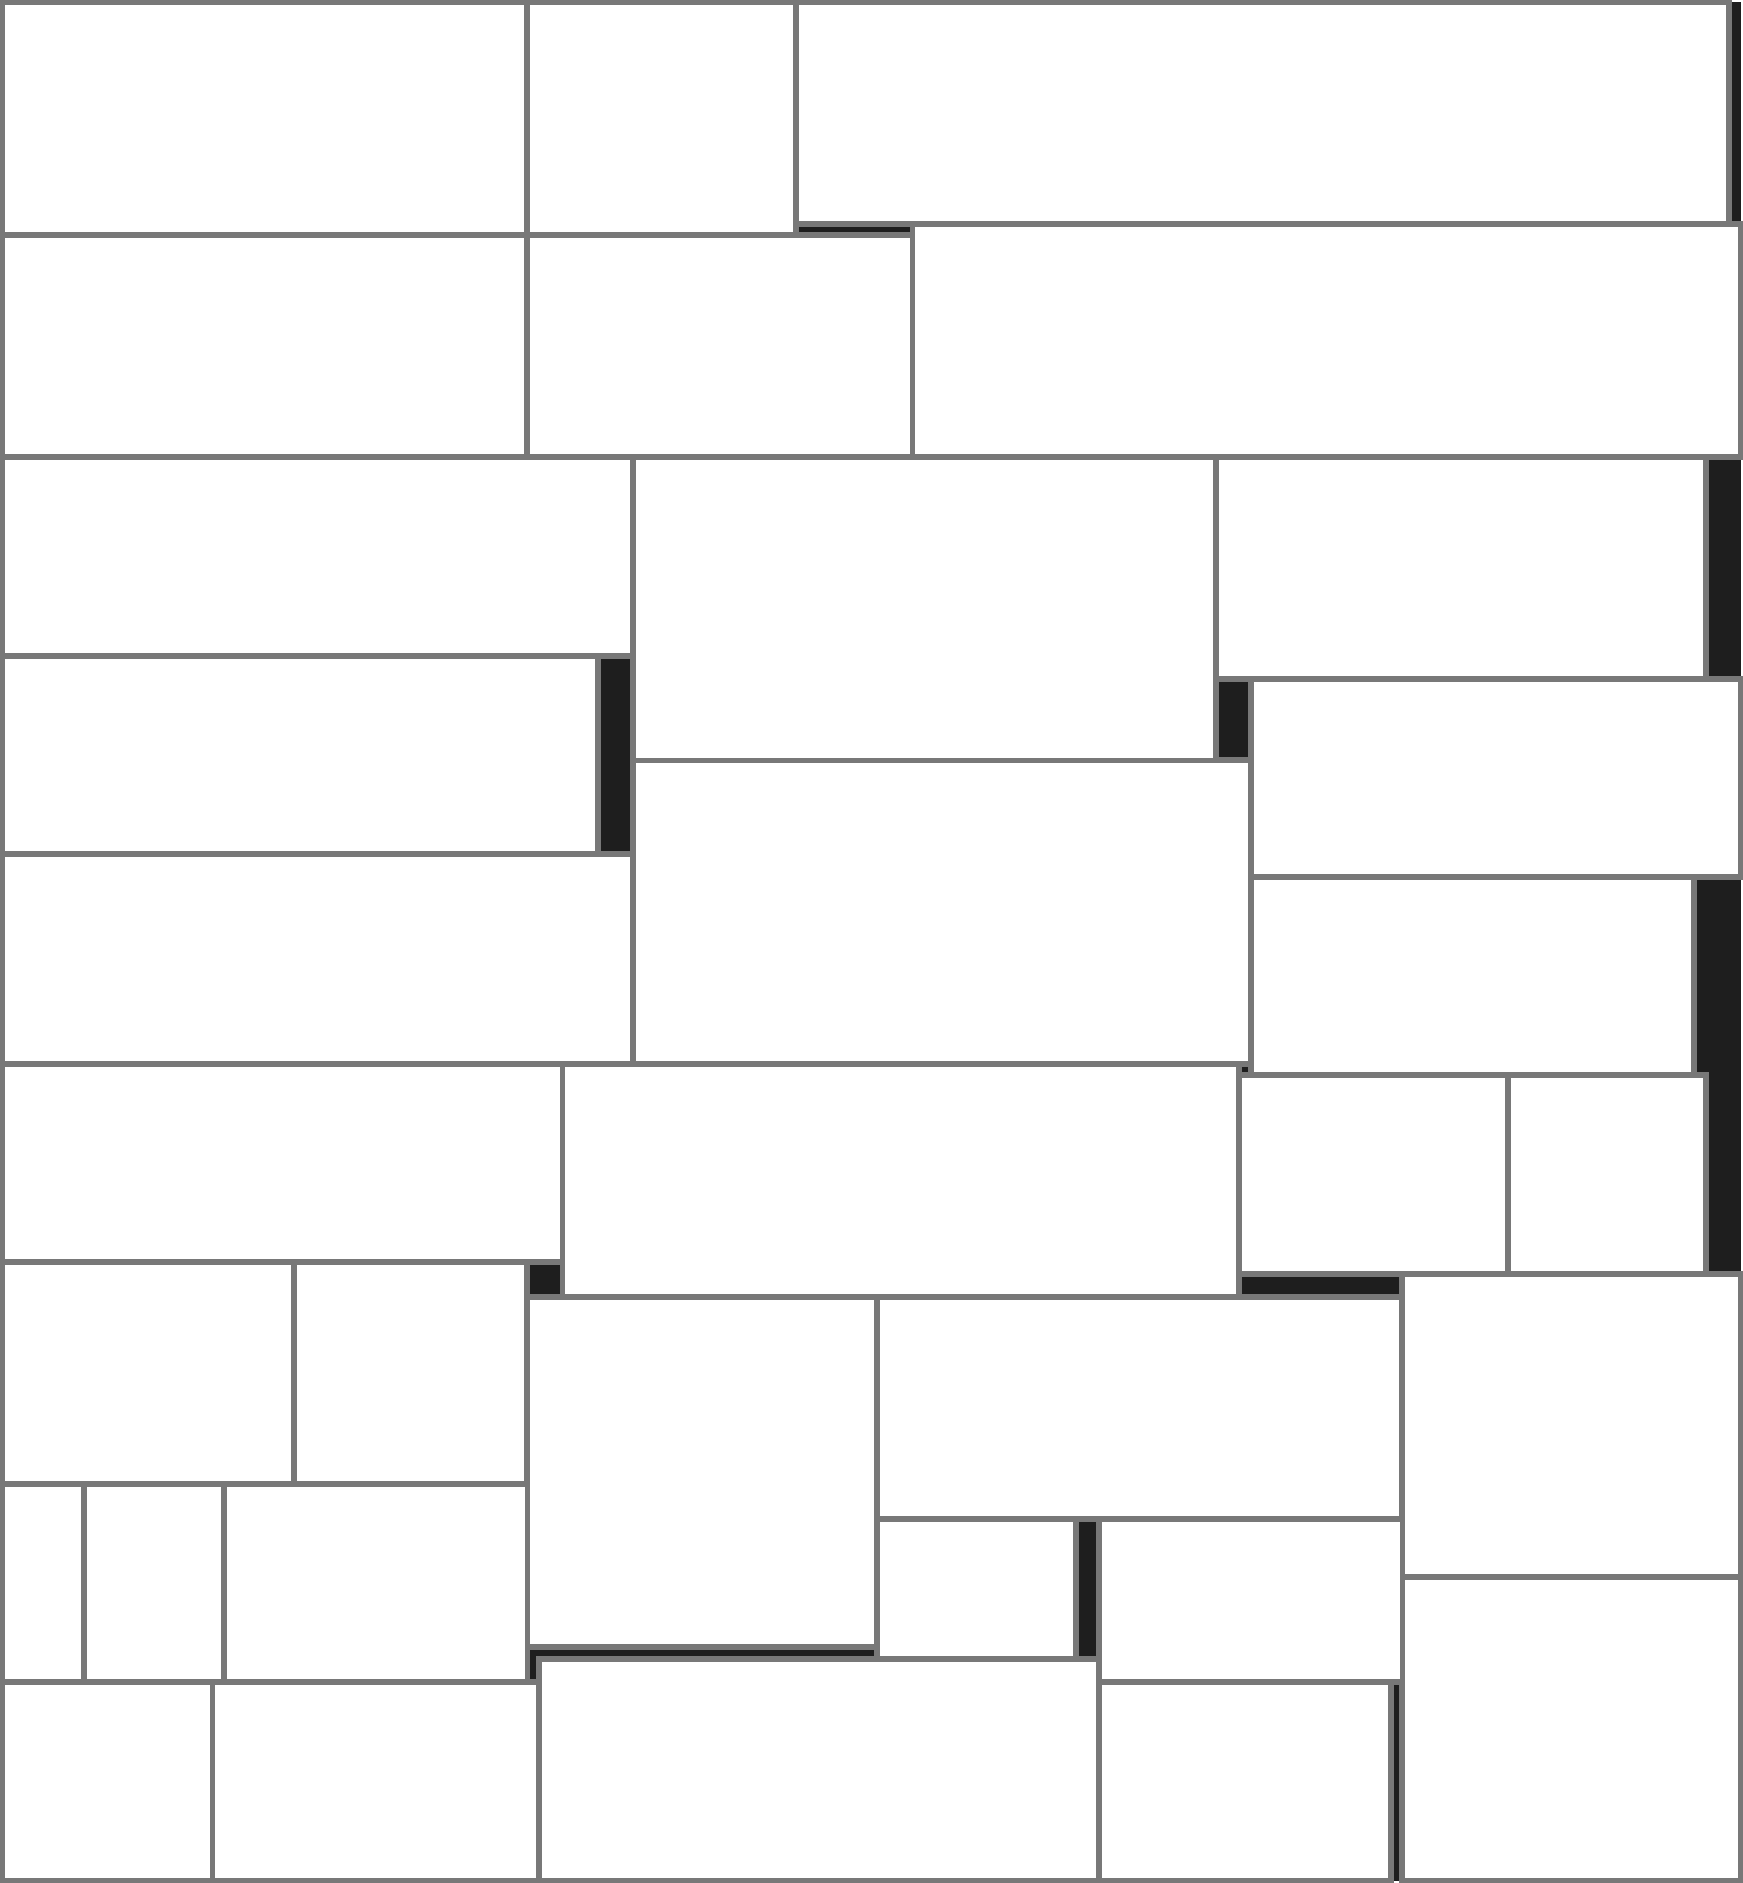
\includegraphics[angle=90,width=.47\textwidth]{ami33}} \hfill
\subfloat[ami49 (2.1\% dead)]{\includegraphics[angle=90,width=.47\textwidth]{ami49}} \\
\subfloat[xerox (2.3\% dead)]{\includegraphics[width=.6\textwidth]{xerox}} \\
\caption{The best solutions of MCNC benchmarks found}
\label{fig:mcnc}
\end{figure}

\section{Comparsion with Recent Algorithms}

The algorithm implemented was compared with some of recent algorithms in the field and to the previous work by author \cite{vh}, which uses the same optimisation framework but different representation (slicing tree). Results of this comparsion are shown on Table~\ref{tab:bachelor}. Unfortunately, getting and comparing the results is hard, because every article uses different benchmarks and watches different floorplan measures (e.g. total area instead of unused area). Also the time is given for rough estimation only, as the tests were performed on different machines. Our configuration was run at 2~GHz CPU. Results are shown on Table~\ref{tab:stateofart}. Both short run ($I=2000,G=1000$) and long run ($I=50000,G=1000$) of the algorithm are shown.

\begin{table}
\centering
\begin{tabular}{|r|c|c|c|c|}
\hline
Test & \multicolumn{2}{|c|}{POEMS/Slicing (unused area, time)} & \multicolumn{2}{|c|}{POEMS/B*-Tree (unused area, time)} \\
\hline
\hline
n100 & {\bf 11,142} & 3,741,504 ms & {\bf 5,761} & 1,575,026 ms \\
\hline
n200 & {\bf 17,636} & 8,500,771 ms & {\bf 8,136} & 3,041,565 ms \\
\hline
\end{tabular}
\caption{Comparsion with the previous work}
\label{tab:bachelor}
\end{table}

\begin{table}
\centering
\begin{tabular}{|r|c|c|c|c|c|}
\hline
 & \multicolumn{2}{|c|}{POEMS/B*-Tree} & CompaSS & B*-Tree & B*-Tree/SA \\
\hline
Test & long run & short run & see \cite{bench} & see \cite{btree} & see \cite{btreesa} \\
\hline
\hline
apte & 0.78\% (969 s) & 0.78\% (76 s) & 0.78\% (0 s) & {\bf 0.77\%} (7 s) & 1.59\% (2 s) \\
\hline
xerox & {\bf 2.30\%} (902 s) & 3.00\% (71 s) & 3.45\% (16 s) & 2.48\% (25 s) & 3.85\% (5 s) \\
\hline
hp & 3.88\% (1,927 s) & 5.57\% (79 s) & 2.28\% (3 s) & {\bf 1.35\%} (55 s) & 4.47\% (20 s) \\
\hline
n100 & {\bf 1.98\%} (4,826 s) & 4.79\% (306 s) & 7.32\% (4 s) & N/A & N/A \\
\hline
n200 & {\bf 3.68\%} (8,408 s) & 6.89\% (552 s) & 6.48\% (10 s) & N/A & N/A \\
\hline
\end{tabular}
\caption{Comparsion with recent algorithms}
\label{tab:stateofart}
\end{table}

\clearpage
\section{Conclusions}
\label{sec:conclusions}

\subsection{Outcomes}

A brand new solver for the 2D rectangle packing problem (floorplanning) was designed, implemented and tested. It is based on the POEMS iterative optimisation framework and genetic algorithm, used for local search. The best-fit inspired heuristic was used in order to create the prototype solution of each problem and 6 different actions for modifying it. 

The algorithm was implemented in the Java programming language version 1.6 and tested on public benchmark data available on the website \cite{bench} (GSRC \cite{benchgsrc}, MCNC \cite{benchmcnc}). The results were compared to the author's previous work \cite{vh} and to some of the state-of-the-art algorithms. It was very difficult to compare all algorithms as most of them have multiple setup parameters that significantly influence the solution quality and the computation time.

The experiments show that the suggested algorithm is competetive in quality, and even slightly better than all the other algorithms tested. Its performance is strongly dependent on the iteration and generation count, so the timing constraints must be taken into account. If the result quality is critical and the computation time not limited, the proposed algorithm is a good choice. It outperforms CompaSS \cite{bench} and B*-Tree/SA \cite{btreesa} in all benchmarks. Usually, in about 1 hour, satisfactory to very good results are acquired. If the result quality is not crucial, a setup running for several minutes can be sufficient for solving smaller problem instances.

The new algorithm was also compared to the previous work by the author \cite{vh}. The best results from the previous work and the second best results were taken from the current implementation (as the time magnitude is similar). For both benchmarks, the performance of the new algorithm is roughly twice as good and the result was obtained twice as fast.

\subsection{Further Work}

Further development of the algorithm could include dealing with pre-placed or soft modules. Another advantage of the B*-Tree is that it can be quite easily extended to work with rectilinear modules (for instance, T-shaped or L-shaped modules). That can be done by splitting these rectilinear shapes into rectangles and modifying the placing algorithm to keep those corresponding rectangles compacted. Several articles that work with this solution have already been published.

Another extension possibility is to add support for placing and optimising soft modules. This change can be implemented, for example, by adding a `ratio' parameter to each B*-Tree node, which is optimised too. This parameter is kept to stay in the range specified by the problem assignement (usually, the problems specify the minimum and the maximum ratio allowed for each module).

Finally, the most versatile floorplan optimiser would support both of these extensions mentioned above. The combination is not simple, as it is difficult to specify the ratio range of a general rectilinear module (the problem is to specify the meaning of the `ratio' itself).

Optimisation of the wirelength is easy to add, too. A different loading procedure for the input data must be implemented and the fitness function calculation must be changed, and that is all. And, perhaps, the function for creating of a prototype could be also changed to take interconnection into account.

\chapter{Using of the Program}
\label{sec:usage}

\section{Command Line Usage}

Program is distributed as a standalone console application that transforms input (problem assignment) into the output (problem solution). As the application is an experimental academic project only, it is aimed to be used by an experienced computer user via the console. Usage was tailored to support benchmarking easily.

The program takes nine arguments and all of them are mandatory. If any argument is missing, program shows usage and exits. Table~\ref{tab:args} contains all the arguments with their descriptions as well as common values for convenience.

The input directory must contain text files with benchmarks in the correct format (see further), the output directory must be writable. For each benchmark file, an output sub directory will be created that will be filled with the results, the statistic and with other information about the computation process. Most of the files created there are meant for testing or benchmarking purposes only. The most important file is the {\tt floorplan.svg}, that shows the final and best result found in the graphical form.

\begin{verbatim}
run.jar IN OUT VERBOSE R I G N S BESTFIT
run.jar benchmark/ benchmark/result/ false 1 1000 500 5 50 true
\end{verbatim}

\begin{table}
\begin{center}
\begin{tabular}{|l|l|l|}
\hline
Name & Description & Common value \\
\hline
\hline
{\tt IN} & input directory name & benchmark/ \\
\hline
{\tt OUT} & output directory name & benchmark/result/ \\
\hline
{\tt VERBOSE} & verbose mode enabled & false \\
\hline
{\tt R} & number of runs for each benchmark & 1 \\
\hline
{\tt I} & iteration count & 1000 \\
\hline
{\tt G} & generation count & 500 \\
\hline
{\tt N} & niché count (same as action sequence length) & 5 \\
\hline
{\tt S} & niché size (same as number of individuals in niché) & 50 \\
\hline
{\tt BESTFIT} & best-fit prototype creation & true \\
\hline
\end{tabular}
\end{center}
\caption{Program command line arguments}
\label{tab:args}
\end{table}

\section{Benchmark File Format}

This section describes how the benchmark files are written. All benchmarks were downloaded from the official website of the free Parquet placer \cite{bench} and the benchmark format was preserved unchanged for convenience.

The benchmark file is a plain text file. The file starts with a single integer specifying the number of modules that are further specified in the file. Then the file continues with a sequence of float pairs split by a space which specifies the dimensions of individual modules. Although the dimensions are - in fact - real, they can be cast to integers, as their fraction parts are equal to zero.

As an example, the whole MCNC HP benchmark is listed in Fig.~\ref{fig:hpcode}

\begin{figure}
\begin{minipage}{\textwidth}
\begin{verbatim}
11 
1036.00 462.00 
378.00 700.00 
980.00 210.00 
980.00 210.00 
980.00 210.00 
3304.00 546.00 
3304.00 546.00 
2016.00 252.00 
3080.00 462.00 
2016.00 252.00 
3080.00 462.00 
\end{verbatim}
\end{minipage}
\caption{HP benchmark plain text code}
\label{fig:hpcode}
\end{figure}

\section{CD Contents}

The included CD, there is a complete source code for both algorithm implementation and the thesis (for the Table of Contents, please refer to Table~\ref{tab:cd}). Basically, it is an snapshot image of the repository. In case that the CD is lost, source codes can be found on the internet. The website that hosts the complete project repository can be found here \cite{repository}.

\begin{table}
\begin{center}
\begin{tabular}{|l|l|l|}
\hline
Name & Description \\
\hline
\hline
{\tt benchmark/} & all collected benchmarks \\
\hline
{\tt src/} & program source code \\
\hline
{\tt test/} & program unit tests source code \\
\hline
{\tt thesis/} & thesis and figures source code \\
\hline
\end{tabular}
\end{center}
\caption{Included CD disc contents}
\label{tab:cd}
\end{table}

\begin{thebibliography}{1}

\bibitem{vh}
{V.~Hordějčuk:
{\em Optimisation of Rectangular Shapes Placement by Means of Evolutionary Algorithms},
bachelor`s thesis,
2010.}

\bibitem{hynek}
{J.~Hynek:
{\em Genetické algoritmy a genetické programování},
Grada Publishing, a.s.,
2008.}

\bibitem{btreesa}
{T.C.~Chen, Y.W.~Chang:
{\em Modern Floorplanning Based on B*-Tree and Fast Simulated Annealing},
IEEE Trans. Computer-Aided Design of Integrated Circuits and Systems, Vol. 24, No. 4, pp. 637--650,
April 2006.}

\bibitem{poems}
{J.~Kubalik, J.~Faigl:
{\em Iterative Prototype Optimisation with Evolved Improvement Steps},
Lecture Notes in Computer Science, Springer,
2006.}

\bibitem{tcg}
{J.M.~Lin, Y.W.~Chang:
{\em TCG: A Transitive Closure Graph-Based Representation for Non-Slicing Floorplans},
IEEE Trans. Very Large Scale Integration System, Vol. 13, No. 2, pp. 288--292,
February 2005.}

\bibitem{tcgs}
{J.M.~Lin, Y.W.~Chang:
{\em TCG-S: Orthogonal Coupling of P*-admissible Representations for General Floorplans},
IEEE Trans. Computer-Aided Design of Integrated Circuits and Systems, Vol. 23, No. 6, pp. 968--980,
June 2004.}

\bibitem{pe2}
{M.~Lai and D.F.~Wong:
{\em Slicing Tree Is a Complete Floorplan Representation},
Proceedings of Design Automation Conference, pp. 228--232,
2001.}

\bibitem{btree}
{Y.C.~Chang, Y.W.~Chang, G.M.~Wu, S.W.~Wu:
{\em B*-Trees: A New Representation for Non-Slicing Floorplans},
Proceedings of 36th Design Automation Conference, pp. 458--463,
2000.}

\bibitem{cbl}
{X.L.~Hong, G.~Huang, T.~Cai, J.~Gu, S.~Dong, C.K.~Cheng, J.~Gu:
{\em Corner Block List: An Effective and Efficient Topological Representation of Non-Slicing Floorplan},
Proceedings of International Conference on Computer Aided Design, pp. 8--12, 
2000}

\bibitem{otree}
{P.N.~Guo, C.K.~Cheng, T.~Takahashi, T.~Yoshimura:
{\em Floorplanning Using a Tree Representation},
IEEE Transactions on Computer-Aided Design of Integrated Circuits and Systems, vol. 20, no. 2, pp. 281--289, 
February 2001.}

\bibitem{sp}
{H.~Murata, K.~Fujiyoshi, S.~Nakatake, Y.~Kajitani:
{\em VLSI Module Placement Based on Rectangle-Packing by the Sequence-Pair},
IEEE Transactions on Computer-Aided Design of Integrated Circuits and Systems, vol. 15, no. 12, pp. 1518--1524, 
1996.}

\bibitem{bsg}
{S.~Nakatake, K.~Fujiyoshi, H.~Murata, Y.~Kajitani:
{\em Module Placement on BSG-structure and IC Layout Applications},
Proceedings of International Conference on Computer Aided Design, pp. 484--491, 
1996.}

\bibitem{nphard}
{H.~Murata, K.~Fujiyoshi, S.~Nakatake, Y.~Kajitani:
{\em VLSI Module Placement Based on Rectangle-Packing by the Sequence-Pair},
1996.}

\bibitem{koza}
{J.R.~Koza:
{\em Genetic Programming. On the Programming of Computers by Means of Natural Selection},
Cambridge, MA: MIT Press,
1992.}

\bibitem{tournament}
{D.E.~Goldberg, K.~Deb:
{\em A Comparative Analysis of Selection Schemes Used in Genetic Algorithms},
Foundations of genetic algorithms, Bloomington, IN,
1991.}

\bibitem{pe}
{D.F.~Wong, C.L.~Liu:
{\em A New Algorithm for Floorplan Design},
Proceedings of Design Automation Conference, pp. 101--107,
1986.}

\bibitem{amir}
{B.S.~Baker, E.G.~Coffman, R.L.~Rivest:
{\em Orthogonal Packings in Two Dimensions},
SIAM Journal on Computing, vol. 9, no. 4, pp. 846--855,
1980.}

\bibitem{ga}
{J.H.~Holland:
{\em Adaptation in Natural and Artificial Systems},
Michigan Press, 
1975.}

\bibitem{darwin}
{C.~Darwin:
{\em O vzniku druhů přirozeným výběrem čili zachování vhodných odrůd v boji o život},
F. Klapálek, Praha, 
1914.}

\bibitem{bench}
{\tt http://vlsicad.eecs.umich.edu/BK/FPUtils/}

\bibitem{benchmcnc}
{\tt http://vlsicad.eecs.umich.edu/BK/CompaSS/results/mcnc\_opt.html}

\bibitem{benchgsrc}
{\tt http://vlsicad.eecs.umich.edu/BK/CompaSS/results/gsrc\_opt.html}

\bibitem{repository}
{\tt http://code.google.com/p/vh-master-thesis/}

\end{thebibliography}


% Seznamy obrázků a tabulek
% =========================

\listoffigures
\listoftables

% Konec dokumentu
% ===============

\end{document}
